% final draft
% todo: Interkapitel-Referenzen, Kontextgrafik, Qualitiative Fragebogen-Daten für Hypothese Kooperation


\chapter{Evaluierung der erstellten Modelle} % (fold)
\label{cha:eval_modell}

Im zweiten Teil der Evaluierung wird nicht der Umgang mit dem Werkzeug betrachtet (siehe dazu Kapitel \ref{cha:eval_werkzeug}), sondern auf das unmittelbare Resultat der Werkzeugverwendung, also das erstellte Modell eingegangen. Ebenfalls nicht Gegenstand der Untersuchung ist in diesem Abschnitt die Wirkung der Modellbildung auf die operative Arbeit („Production Work“), die in Kapitel \ref{cha:eval_aw} betrachtet wird. Abbildung \ref{fig:img_Kontextgrafiken_k13} stellt dieses Kapitel und dessen Aufbau im Kontext der anderen inhaltlich vor- und nachgelagerten Kapitel dar.


\begin{figure}[htbp]
	\centering
		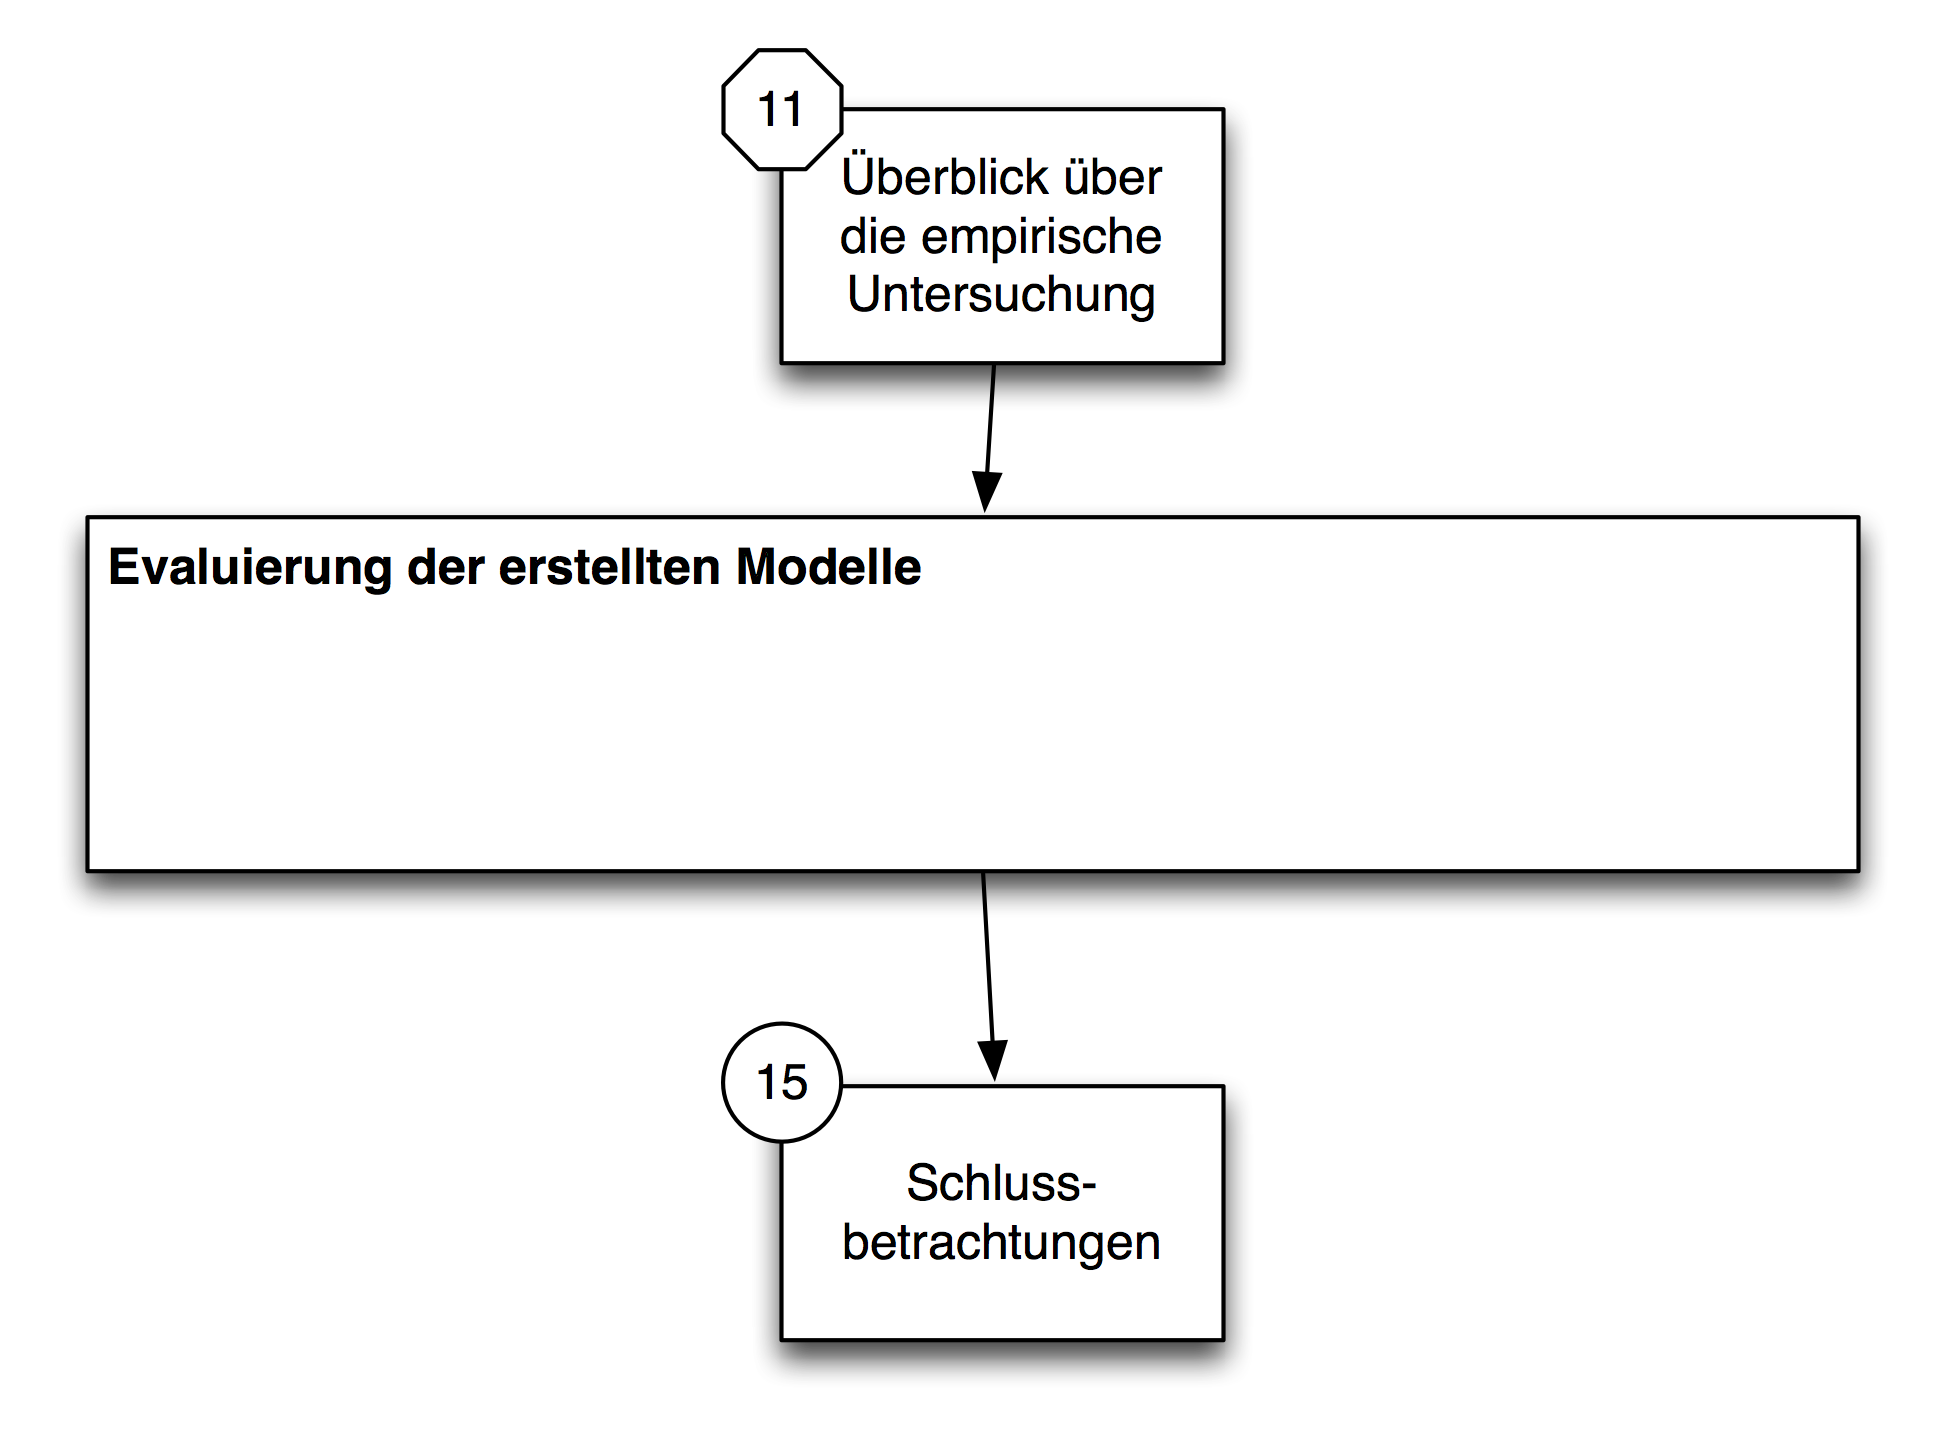
\includegraphics[scale=0.6]{img/Kontextgrafiken/k13.png}
	\caption{Kapitel „Evaluierung der erstellten Modelle“ im Gesamtzusammenhang}
	\label{fig:img_Kontextgrafiken_k13}
\end{figure}


Ausgehend von den erstellten Modellen und deren Entstehungsprozess wird also in diesem Kapitel untersucht, wie das Werkzeug auf die in dieser Arbeit gewählte Form der Unterstützung expliziter „Articulation Work“, nämliche der kooperativen Externalisierung und Abstimmung mentaler Modelle, wirkt. Dementsprechend sind die im folgenden Abschnitt beschrieben Hypothesen aus den Ausführungen der Kapitel über mentale Modelle (Kapitel \ref{cha:mentale_modelle}) und der Methodik zur Externalisierung derselben (Kapitel \ref{cha:methodik}) abgeleitet. 

Zusätzlich wird eine explorativ gebildete Hypothese untersucht, die sich auf inhaltlicher Ebene mit dem Phänomen der Abbildung von Zusammenhängen durch räumliche Konfiguration der Konzepte in einem Modell beschäftigt, das in der Untersuchung der Hypothese \ref{hyp:diagmodelle} bereits hinsichtlich der Werkzeugverwendung beschrieben wurde.

\section{Hypothesen} % (fold)
\label{sec:m_hypothesen}

In diesem Abschnitt werden die Hypothesen abgeleitet, die in diesem Kapitel geprüft werden. Wie in Kapitel \ref{cha:eval_werkzeug} ist zwischen konzeptuell aus der Aufgabenstellung bzw. der entwickelten Methodik abgeleiteten Hypothesen über die Wirkung des Werkzeugs und explorativ während der Evaluierung selbst gebildeten Hypothesen über Eigenschaften des Werkzeugs bzw. dessen Verwendung im Kontext der Modellbildung zu unterscheiden.

\subsection{Konzeptuell begründete Hypothesen} % (fold)
\label{sub:m_konzeptionell_begründete_hypothesen}

Die folgenden Hypothesen sind aus der Aufgabenstellung bzw. den Ausführungen zur Modellierungs-Methodik abgeleitet. Auf die entsprechenden Ausführungen in den Kapiteln \ref{cha:mentale_modelle} bzw. \ref{cha:methodik} wird jeweils bei der Begründung der Hypothesen verwiesen.

Ein wesentlicher Aspekt bei der Externalisierung mentaler Modelle ist die Offenheit der Repräsentationssprache. Diese ist aus Abschnitt \ref{sub:concept_mapping} begründbar und in Anforderung \ref{anf:nicht_vorgegebene_semantik_der_modellierungselemente} abgebildet. Unter „Offenheit“ ist in diesem Zusammenhang die Eigenschaft der Repräsentationssprache gemeint, keine vordefinierte Semantik der Modellelemente vorzugeben sondern diese von den Modellierenden festlegen zu lassen. Dies umfasst im vorliegenden Fall sowohl die Bedeutung der unterschiedlichen Konzepttypen als auch die Bedeutung der Verbindungen zwischen Konzepten. Das Werkzeug darf also in diesem Zusammenhang die Benutzer nicht bei der Wahl der Repräsentationskonzepte und damit bei der Externalisierung selbst einschränken. Die Prüfung dieser Hypothese ermöglicht die Beurteilung der Erfüllung der Anforderung \ref{anf:nicht_vorgegebene_semantik_der_modellierungselemente} (siehe Seite \pageref{anf:nicht_vorgegebene_semantik_der_modellierungselemente}).

\begin{hyp}
	\label{hyp:keine_einschränkung}
	Das Werkzeug schränkt Benutzer semantisch nicht bei der Externalisierung ihrer mentalen Modelle ein.
\end{hyp}

Das Argument der Nicht-Beschränkung der Benutzer bei der Externalisierung hat neben der eben beschriebenen Sprach-Dimension auch eine konkrete Modell-Dimension. Während sich obige Hypothese auf semantische Einschränkungen der Externalisieungsmöglichkeiten bezieht, ist sind auch konkrete, strukturelle Einschränkungen bei der Verwendung des Werkzeugs zur Externalisierung eines bestimmten mentalen Modells zu berücksichtigten. Die Externalisierung muss -- um nicht beschränkend zu wirken -- beliebig umfangreiche Modelle ermöglichen. „Umfangreich“ bedeutet hier, dass das Modell beliebig viele Elemente enthalten können muss und diese beliebig untereinander in Beziehung gesetzt werden können. Die Prüfung dieser Hypothese ermöglicht die Beurteilung der Erfüllung der Anforderung \ref{anf:bearbeitung_von_beliebig_komplexen_modellen} (siehe Seite \pageref{anf:bearbeitung_von_beliebig_komplexen_modellen}).
	
\begin{hyp}
	\label{hyp:beliebige_komplexität}
	Das Werkzeug ermöglicht die Repräsentation beliebig umfangreicher Modelle.
\end{hyp}

Die Möglichkeit durch die Entstehungsgeschichte des erstellten Modells zu navigieren ist eine Funktion, die ebenfalls hinsichtlich ihrer Wirkung auf die Externalisierung mentaler Modelle untersucht werden muss. In der dieser Funktionalität zugrunde liegenden Literatur (\citep{Shipman00}, \citep{Klemmer02}) wird diese als wesentlich bezeichnet, wenn Externalisierungsprozesse unterbrochen werden, kooperativ durchgeführt werden oder Dritten die Möglichkeit gegeben werden soll, die Entstehung des Modells nachzuvollziehen. Allen drei Aspekten liegt die Annahme zugrunde, dass in der Historie des Externalisierungsprozesses die dem Ergebnis zugrunde liegenden Ideen und Annahmen zu erkennen sind. Im Kontext dieser Arbeit bedeutet dies, dass aus der Nachverfolgung der Historie des externalisierten Modells die diesem zugrunde liegenden mentalen Modelle verständlich und nachvollziehbar werden. Die Prüfung dieser Hypothese ermöglicht die Beurteilung der Erfüllung der Anforderung \ref{anf:persistente_ablage_des_modells_möglichkeit_zur_rekonstruktion} (siehe Seite \pageref{anf:persistente_ablage_des_modells_möglichkeit_zur_rekonstruktion}).

\begin{hyp}
	\label{hyp:historie}
	Die Reflexion des Modellierungsverlaufs ermöglicht das Verständnis der im dem Modell repräsentierten Inhalte.
\end{hyp}

Die Externalisierung mentaler Modelle mit Hilfe von computer-gestützten Werkzeugen ist keine originäre Idee dieser Arbeit. Computerunterstützung existiert vor allem im Bereich des „Concept Mapping“ (siehe Abschnitt \ref{sub:concept_mapping}), das methodisch maßgeblich in das vorgeschlagene Vorgehen des hier vorgestellten Ansatzes einfließt (siehe Kapitel \ref{cha:methodik}). In den existierenden Werkzeugen werden jedoch die kooperative Erstellung und kommunikative Validierung der externalisierten Modelle nicht explizit berücksichtigt. Beide Aspekte sind jedoch -- wie bei der Beschreibung der Strukturlegetechniken \ref{sub:strukturlegetechniken} ausgeführt -- wichtig für den Abgleich mentaler Modelle und damit für die erfolgreiche Durchführung von „Articulation Work“. Die Ermöglichung und Stärkung der Kooperation der Beteiligten untereinander ist also ein wesentlicher Teilaspekt der Anforderung \ref{anf:kollaborative_und_unmittelbare_manipulierbarkeit_des_modells} an das Werkzeug („Kooperative und unmittelbare Manipulierbarkeit des Modells“). Die Prüfung dieser Hypothese ermöglicht die Beurteilung der Erfüllung der Anforderung \ref{anf:kollaborative_und_unmittelbare_manipulierbarkeit_des_modells} (siehe Seite \pageref{anf:kollaborative_und_unmittelbare_manipulierbarkeit_des_modells}).

\begin{hyp}
	\label{hyp:stärkere_kooperation}
	Die Verwendung des Werkzeugs führt zu stärkerer Kooperation bei der Modellerstellung als die Verwendung von bildschirm-basierten Werkzeugen.
\end{hyp}

Hinsichtlich der in Kapitel \ref{cha:anforderungen} formulierten Anforderungen können die hier formulierten Hypothesen zusammenfassend wie in Tabelle \ref{tab:hyp_modell} dargestellt eingeordnet werden.

\begin{table}[htbp]
	\centering
	\caption{Hypothesen zur Modellbildung und deren Bezug zu den Anforderungen an das Werkzeug}
\begin{tabular}{|c|c|}
  \hline
   Hypothese & Anforderung \\ \hline
   \ref{hyp:keine_einschränkung} & \ref{anf:nicht_vorgegebene_semantik_der_modellierungselemente} \\
   \ref{hyp:beliebige_komplexität} & \ref{anf:bearbeitung_von_beliebig_komplexen_modellen} \\
   \ref{hyp:historie} & \ref{anf:persistente_ablage_des_modells_möglichkeit_zur_rekonstruktion} \\
   \ref{hyp:stärkere_kooperation} & \ref{anf:kollaborative_und_unmittelbare_manipulierbarkeit_des_modells} \\ \hline
\end{tabular} 
	\label{tab:hyp_modell}
\end{table}

% subsection konzeptionell_begründete_hypothesen (end)

\subsection{Explorativ gebildete Hypothesen} % (fold)
\label{sub:m_explorativ_gebildete_hypothesen}

Im Verlauf der beiden Evaluationen war die Herstellung von Verbindungen zwischen Modellelementen aus technischen Gründen schwierig zu benutzen und sehr anfällig für Fehlfunktionen. Dies führte dazu, dass Verbinder nahezu nicht verwendet wurden (siehe dazu die Auswertungen zu Hypothese \ref{hyp:diagmodelle} in Abschnitt \ref{sub:repräsentation_diagrammatischer_modelle}). In dieser Situation wurden Beziehungen zwischen Modellelementen von den Benutzern durch die räumliche Anordnung der Elemente ausgedrückt. Diese implizite Darstellung von relationaler Information erfolgte in allen Fällen spontan und ohne Anleitung oder Instruktion. Dies führte zu der Vermutung, dass die Verwendung von Verbindern zur Abbildung von Beziehungen bzw. Zusammenhängen zwischen Elementen nicht notwendig ist. Um diese Vermutung zu prüfen, wurde sie formal als Hypothese \ref{hyp:keine_verbinder} in die Untersuchung aufgenommen.

\begin{hyp}
	\label{hyp:keine_verbinder}
	Zur Abbildung von Zusammenhängen ist die Verwendung von Verbindern nicht notwendig.
\end{hyp}

% subsection explorativ_gebildete_hypothesen (end)

% section hypothesen (end)

\section{Untersuchungsdesign und Durchführung} % (fold)
\label{sec:m_untersuchungsdesign}

In diesem Abschnitt wird auf Basis der oben formulierten Hypothesen das Untersuchungsdesign abgeleitet und die Durchführung der Untersuchung beschrieben. Der erste Teil des Abschnitts beschreibt die Operationalisierung der Hypothesen und damit die Festlegung wie diese konkret geprüft werden können. Im zweiten Teil des Abschnitts wird die Durchführung der Prüfung beschrieben. Hier erfolgt neben der Zuordnung der einzelnen Evaluierungsblöcke (siehe Abschnitt \ref{sec:globales_untersuchungsdesign}) auch die Darstellung rein beschreibender Modell-Parameter, die nicht unmittelbar in die Prüfung der Hypothesen eingehen. 

\subsection{Operationalisierung} % (fold)
\label{sub:m_operationalisierung}

In diesem Abschnitt wird für jede Hypothese identifiziert, in welcher Form sie geprüft werden kann. Dies umfasst die Festlegung der Messpunkte sowie der jeweiligen Mess- und Auswertungsmethode (letzte bezugnehmend auf den in Abschnitt \ref{sec:eingesetzte_werkzeuge_und_verfahren} beschriebenen Verfahren). Zudem werden jene Evaluationsblöcke festgelegt, die für die jeweilige Untersuchung herangezogen wurden.

Für jede Hypothese wird also spezifiziert, anhand welcher Aspekte diese geprüft werden kann (= abhängige Variablen). Zudem wird festgelegt welche Ausgangssituation bei der Anwendung gewählt werden muss, um die Prüfung durchführen zu können (= unabhängige Variable) und welche Faktoren die Beurteilung ggf. ungewollt beeinflussen können (= Störvariablen).

\subsubsection{Keine semantische Einschränkung der Externalisierung} % (fold)
\label{ssub:keine_semantische_einschränkung_der_externalisierung}

Gegenstand dieses Abschnitts ist die Prüfung der Hypothese \ref{hyp:keine_einschränkung}. Diese bezieht sich auf die geforderte Eigenschaft des Werkzeugs, die Benutzer bei der Modellierung semantisch nicht einzuschränken.

Voraussetzung für die Prüfung dieser Hypothese ist die Verwendung des Werkzeugs zur Modellbildung bei einer Aufgabe, die die semantischen Kategorien der Strukturierung nicht vorgibt. In der eingesetzten Methodik wird die Festlegung von Elementtypen explizit gefordert (Vorgehen und Zeitpunkt dafür werden jedoch nicht vorgegeben). Etwaige Modellierungsvorkenntnisse können diese Festlegung insofern beeinflussen, als dass die Konzepte bekannter Sprachen bevorzugt eingesetzt werden könnten. Im Sinne der Hypothese ist dies jedoch keine Störvariable, da die Forderung nach nicht einschränkender Struktur auch die Verwendung existierender Modellierungssprachen umfassen muss.

Die nicht einschränkende Wirkung kann qualitativ anhand von Benutzeraussagen und dem Prozess und Ergebnis der Modellentstehung beurteilt werden. Im ersten Fall bieten sich neben der direkten Frage nach der Abbildbarkeit der gewünschten Information auch Teilaspekte des \gls{PMS}-Framework \citep{Sedera02} an, das unter anderem die subjektiv wahrgenommene Qualität des Modellierungsergebnisses und die Abbildbarkeit der subjektiv wichtigen Information im Modell abbildet (zur Eignung des \gls{PMS}-Frameworks im Kontext dieser Arbeit siehe \citep{Wahlmuller10}). Am Prozess- und Ergebnis der Modellentstehung selbst kann beurteilt werden, ob und inwieweit die zur Verfügung gestellten, semantisch nicht vorbelegten Modellierungselemente für die Abbildung der gewünschten Information ausreichend bzw. geeignet waren. Dazu kann betrachtet werden, ob die beschränkte Anzahl von Elementen im Verlauf der Modellierung zu verändertem Vorgehen in der Abbildung oder zur Nichtabbildung bestimmter Modellaspekte führte und ob durch semantische Mehrfachbelegung bzw. die Einführung von nicht als Modellierungselement vorgesehenen Bausteinen der Sprachumfang über das ursprünglich intendierte Maß hinaus erweitert wurde. 

Vergleichend können zusätzlich Modelle herangezogen werden, die aus identischen Fragestellungen wie jene mit dem Werkzeug erstellten resultieren, bei denen jedoch ein in der Anzahl und Semantik der Modellierungselemente frei erweiterbares Werkzeug zum Einsatz kommt. Hier ist von Interesse, ob die erstellten Modelle semantisch vielfältiger sind als jene, die mit dem hier vorgestellten Werkzeug erstellt wurden.

% subsubsection keine_semantische_einschränkung_der_externalisierung (end)

\subsubsection{Repräsentation beliebig umfangreicher Modelle} % (fold)
\label{ssub:repräsentation_beliebig_komplexer_modelle}

Gegenstand dieses Abschnitts ist die Operationalisierung der Hypothese \ref{hyp:beliebige_komplexität}. Dabei wird überprüft, ob das Werkzeug die Abbildung beliebig umfangreicher Modellierungsaufgaben ermöglicht.

Voraussetzung zur Prüfung dieser Hypothese ist die Verwendung von Modellierungsaufgaben, die zu umfangreichen Modellen führen. Umfangreichen Modellierungsaufgaben sind Aufgaben, die bei detaillierter Modellierung >15 Modellelemente benötigen\footnote{15 wurde als Grenze gewählt, weil diese Anzahl die Obergrenze an gleichzeitig am Werkzeug verwendbaren Elementen darstellt}). Dies ist deshalb notwendig, weil der wesentliche beschränkende Faktor des Umfangs eines Modells am hier vorgestellten Werkzeug die physisch eingeschränkte Größe der Modellierungsoberfläche ist. Etwaige Modellierungsvorkenntnisse der Benutzer sind bei der Prüfung dieser Hypothese nicht von Relevanz.

Um Schlussfolgerungen auf eine etwaig einschränkende Wirkung des Werkzeugs auf den Umfang der Modelle treffen zu können, muss eine entsprechende Aufgabenstellung einerseits mittels dem hier vorgestellten Werkzeug („Experimentalgruppe“) und andererseits mit einem Werkzeug, dass den Umfang der Modellierungsoberfläche nicht begrenzt („Kontrollgruppe“), abgebildet werden. Die Ergebnisse der beiden Gruppen werden dann gegenübergestellt. Falls bei identischer Fragestellung der Umfang der Modelle in der Kontrollgruppe signifikant höher ist als jener der Experimentalgruppe, kann von einer einschränkenden Wirkung ausgegangen werden und die Hypothese müsste abgelehnt werden.

Daneben sind wiederum Aussagen der Benutzer über die Abbildbarkeit umfangreicher Modelle zur Prüfung der Hypothese heranzuziehen. Entsprechende Fragen wurden in den Evaluierungsblöcken 2, 3, 4 und 5 gestellt, wobei die Fragestellungen in den Blöcken 2 und teilweise 4 eher zu nicht umfangreichen Modellen führte, die auf der Oberfläche ausreichend Platz fanden und deshalb hier nicht berücksichtigt werden können.

% subsubsection repräsentation_beliebig_komplexer_modelle (end)

\subsubsection{Reflexion des Modellierungsverlaufs} % (fold)
\label{ssub:reflexion_des_modellierungsverlaufs}

Gegenstand dieses Abschnitts ist die Operationalisierung der Hypothese \ref{hyp:historie}. Dabei wird überprüft, ob die Möglichkeit zur Reflexion des Modellierungsverlaufs das Verständnis der zugrundeliegenen mentalen Modelle ermöglicht bzw. verbessert.

Zur Prüfung dieser Hypothese müssen Modellierungsaufgaben durchgeführt werden, in deren Rahmen die Interpretation eines Modells durch an der Modellbildung nicht beteiligte Personen durchgeführt werden. Wenn diese Interpretation den ursprünglich vom Modellierer repräsentierten Inhalten entspricht, ist die Interpretation als erfolgreich zu bezeichnen. Zu beurteilen ist nun, in wie weit die Möglichkeit zur Wiedergabe des Modellierungsverlaufs bei der Interpretation genutzt wurde und ob diese Nutzung Auswirkungen auf die Interpretation hatte.

Zur Beurteilung wird eine Modellierungssituation geschaffen, in der das Werkzeug zur Externalisierung eines mentalen Modells benutzt wird. In einem zweiten Schritt wird eine weitere, zuvor nicht beteiligte Person aufgefordert, den Inhalt der auf der Modellierungsoberfläche vorhandenen Repräsentation zu interpretieren, wobei der Modellierungsverlauf herangezogen werden darf, eine Interaktion mit dem ursprünglichen Modellierer jedoch nicht gestattet ist. Im dritten Schritt beurteilt der ursprüngliche Modellierer die Adäquatheit der Interpretation und trifft so eine Aussage über den Erfolg des Transfers des mentalen Modells. In Kombination lässt sich eine qualitative Aussage über die Effekte der Historienfunktion treffen.    

% subsubsection reflexion_des_modellierungsverlaufs (end)

\subsubsection{Wirkung auf die Kooperation bei der Modellerstellung} % (fold)
\label{ssub:wirkung_auf_die_kooperation_bei_der_modellerstellung}

Gegenstand dieses Abschnitts ist die Operationalisierung der Hypothese \ref{hyp:stärkere_kooperation}. Gegenstand der Untersuchung ist hier, ob die Verwendung des Werkzeugs bei der Modellbildung zu stärkerer Kooperation zwischen den Beteiligten führt als der Einsatz von bildschirmbasierten Werkzeugen.

Die Prüfung der Wirkung des Werkzeugs auf die kooperative Abbildung von Modellen bedingt Fragestellungen, die Kooperation explizit einfordern. Etwaige Modellierungsvorkenntnisse beeinflussen die Prüfung der Hypothese nicht. Bei der Beurteilung zu berücksichtigen sind etwaige bestehende persönliche Bekanntschaften oder etablierte Gruppen, deren Zusammenarbeit bereits institutionalisiert ist. Um den Einfluss derartiger Faktoren möglichst auszuschließen, müssen die Gruppen bei der Modellbildung zufällig gebildet werden und etwaige Bekanntschaften innerhalb der gebildeten Gruppen explizit im Vorfeld der Untersuchung erhoben werden.

Die hier zu prüfende Hypothese baut auf Hypothese \ref{hyp:kollaborativ} auf. Dort war zu prüfen, ob das Werkzeug kooperatives Arbeiten grundsätzlich ermöglicht. In diesem Abschnitt wird geprüft, ob der Einsatz des Werkzeugs hinsichtlich der Kooperation der Beteiligten tatsächlich einen meßbaren Vorteil gegenüber einem traditionellen, bildschirmbasierten Werkzeug hat. Dazu ist es notwendig, eine vergleichende Untersuchung durchzuführen. Evaluierungsblock 5 wurde dementspechend geplant und umfasste eine die kooperative Abbildung eines Modells sowohl am Modellierungstisch als auch mittels dem bildschirmbasierten Werkzeug CMapTools. Die Aufgabenstellung wurde so gewählt, dass das resultierende Modell grundsätzlich in beiden Werkzeugen abgebildet werden konnte. Untersucht wurde, in welchem Ausmaß Kooperation zwischen den beteiligten Personen auftrat. Als Metriken dienten dazu die Zeitverteilung der Beteiligung am Modellierungsvorgang, der Zeitanteil an Diskussion während der Modellbildung sowie die Anzahl der Initiativwechsel („Turn-Taking“) während eines Durchgangs. Zusätzlich können die Benutzer hinsichtlich des subjektiv empfundenen Ausmaßes der Kooperation sowie der Zufriedenheit mit den im Modell sichtbaren von ihnen selbst eingebrachten Inhalten befragt werden.

Zur Berechnung der Zeitverteilung wird nicht der Zeitanteil der physischen, sondern jener der inhaltlichen Initiative herangezogen. Wo kein die Initiative führender Teilnehmer identifizierbar ist, wird der betreffende Zeitabschnitt zu gleichen Teilen zwischen den Teilnehmern aufgeteilt. Die Zeitverteilung zwischen den Teilnehmern kann dann insofern in die Prüfung einfließen, als dass sehr niedrige oder sehr hohe Zeit-Anteile auf eine unausgewogene Modellierungsbeteiligung hinweisen. Dieses Indiz muss jedoch durch Benutzeraussagen verifiziert werden, da geringe Beteiligung an der Modellierung nicht notwendigerweise auf als mangelhaft empfundene Kooperation hinweist.

Der Zeitanteil an Diskussion während des Modellierungsvorgangs betrifft tatsächlich nur jenen Anteil an der Modellierungsdauer, in dem ein inhaltlicher Austausch zwischen den Teilnehmern im Sinne der Aufgabenstellung stattfindet. Nicht berücksichtigt werden jene Zeiten, in denen das Modell erstellt wird oder in denen nicht im Sinne der Aufgabenstellung gearbeitet wird (etwa bei Fehlfunktionen).

Der Wechsel der Initiative („Turn-Taking“ \citep{Sacks74}) bei der Modellierung bezieht sich im Gegensatz zu der Berechnung der Zeitverteilung zwischen den Teilnehmern auf die physische Initiative bei der Erstellung des Modells. Während in der von \citet{Sacks74} vorgeschlagenen Methodik zur Identifikation von Initiativwechsel auf Konversationen eingegangen wird und damit auf Sprecherwechsel Bezug genommen wird, wird in diesem Fall die Übernahme der physischen Initiative als „Turn“ bezeichnet. Dies erscheint insofern sinnvoll, als das jener Teilnehmer, der die physische Kontrolle über die Eingabemedien besitzt auch exklusiven Zugriff auf die Interaktionsmöglichkeiten mit dem System besitzt und damit potentiell als „Filter“ zwischen den Eingaben der anderen Teilnehmer und der im System repräsentierten Information wirkt.

% subsubsection wirkung_auf_die_kooperation_bei_der_modellerstellung (end)

\subsubsection{Abbildung von Zusammenhängen ohne Verbinder} % (fold)
\label{ssub:abbildung_von_zusammenhängen_ohne_verbinder}

Gegenstand dieses Abschnitts ist die Operationalisierung der Hypothese \ref{hyp:keine_verbinder}. Gegenstand der Untersuchung ist die Beobachtung, dass zur Abbildung von Zusammenhängen die Verwendung von explizit dargestellten Verbindern nicht notwendig ist.

Die Prüfung dieser Hypothese stellt keine Vorbedingungen an die Modellierungsaufgabe oder die Modellierungsvorkenntnisse der Benutzer. Auch können individuelle Anwendungen der Werkzeugs (d.h. nicht nur in kooperativen Szenarien) zur Untersuchung verwendet werden. 

Bei der Prüfung der Hypothese sind zwei Formen der Notwendigkeit von explizit dargestellten Verbindern zu unterscheiden. Zum Einen ist die Notwendigkeit bei der kooperativen Erstellung eines Modells zu untersuchen, bei der sämtliche Beteiligte zu einer einheitlichen Interpretation des dargestellten Modells kommen sollen. Zum Anderen muss auch der Fall einer zeitlich nachgelagerten Interpretation durch Dritte untersucht werden. Hier ist zu erheben, ob die Interpretation der Modellinhalts dem ursprünglichen Verständnis des bzw. der Modellierenden entspricht.

Zur Untersuchung muss dem ursprünglichen Modellierer jeweils eine inhaltliche Interpretation des Modellierungsergebnisses rückgespiegelt werden. Diese Form der kommunikativen Validierung kommt methodisch im Rahmen der Anwendung von Strukturlegetechniken (siehe Abschnitt \ref{sub:strukturlegetechniken}) zum Einsatz und ist deshalb ohnehin Teil der in dieser Arbeit vorgeschlagenen Methodik bei der kooperativen Anwendung des Werkzeugs. Zur zeitlich nachgelagerten Interpretation bedarf es einem separaten Schritt, in dem das Modellierungsergebnis von einer dritten, den der Modellierung nicht beteiligten Person interpretiert und rückgespiegelt wird. 

% subsubsection abbildung_von_zusammenhängen_ohne_verbinder (end)
% subsection m_operationalisierung (end)

\subsection{Durchführung} % (fold)
\label{sub:m_durchführung}

In diesem Abschnitt werden die für diesen Evaluierungs-Teil relevanten deskriptiven Parameter der berücksichtigten Anwendungs-Blöcke angeführt.
Als Grundlage der Überprüfung der Hypothesen werden hier die Evaluierungs-Blöcke 1 bis 5 verwendet. Dabei wurden für die quantitativ zu prüfenden Variablen die Blöcke 2, 3 und 5 herangezogen, da in diesen die größten Stichproben zur Verfügung standen. In die qualitative Auswertung der Ergebnisse wurden hingegen alle Blöcke (1-5) mit einbezogen.

\subsubsection{Stichprobe} % (fold)
\label{ssub:stichprobe}

Für die Untersuchung der Hypothesen in diesem Kapitel wurden die Evaluierungsblöcke 1 bis 5 herangezogen. Die Stichprobe setzt sich wie in Tabelle \ref{tab:stichprobe_modell} beschrieben zusammen.

\begin{table}[htbp]
	\centering
	\caption{Stichproben der Evaluierung zur Modellbildung}

	\begin{tabular}{| l || c | c |}
	\hline
		Evaluierungsblock & $n_{Anwendungen}$ & $n_{Teilnehmende}$ \\ \hline
		technische Evaluierung		  &  9 & 18 \\
		Aushandlung 1 (1. Durchgang)  &  9 & 19 \\
		Aushandlung 1 (2. Durchgang)  &  9 & 18 \\
		Concept Mapping 1			  & 18 & 54 \\
		Aushandlung 2				  & 10 & 13 \\
		Concept Mapping 2 (Tisch)     & 11 & 24 \\
		Concept Mapping 2 (CMapTools) & 12 & 25 \\ \hline
		Gesamt						  & 78 & 171 \\ \hline
\end{tabular}
	\label{tab:stichprobe_modell}
\end{table}
% subsubsection stichprobe (end)

\subsubsection{Modellgröße} % (fold)
\label{ssub:modellgröße}

Die Verteilung der Modellgröße wurde hier anhand der Anzahl der verwendeten Elemente (siehe Abbildung \ref{fig:img_Evaluierung_elementUsageBlocksOverview}) und der Anzahl der verwendeten Verbindungen (siehe Abbildung \ref{fig:img_Evaluierung_elementUsageConnectorsOverview}) dargestellt. Berücksichtigt wurden dabei die Ergebnisse der Evaluierungsblöcke 2 („Aushandlung“) und 3 („Concept Mapping“). Die Modelle der Evaluierungsblöcke 1 und 4 sind aufgrund der uneinheitlichen Aufgabenstellungen nicht vergleichbar, jener Teil des Evaluierungsblocks 5, der mit dem hier vorgestellten Werkzeug durchgeführt wurden, weißt ob der identischen Aufgabenstellung hohe Ähnlichkeit mit den Ergebnissen von Block 3 auf.

\begin{figure}[htbp]
	\centering
		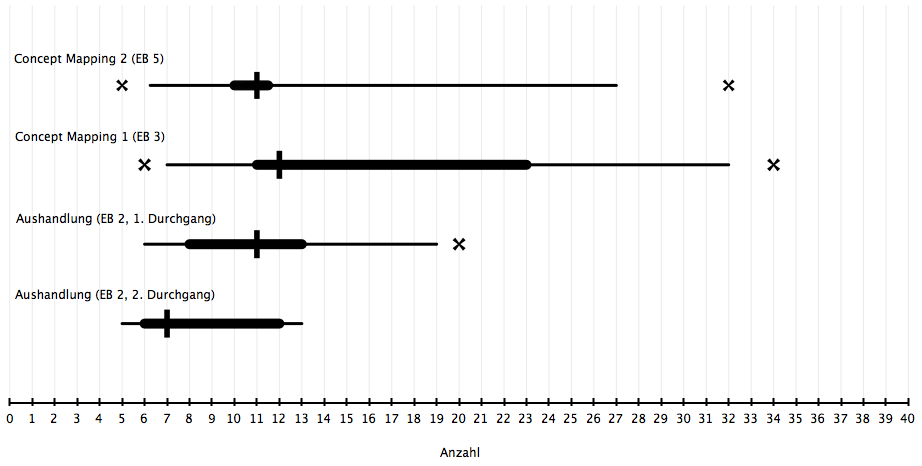
\includegraphics[width=15cm]{img/Evaluierung/elementUsageBlocksOverview.png}
	\caption{Anzahl der verwendeten Elemente -- Übersicht}
	\label{fig:img_Evaluierung_elementUsageBlocksOverview}
\end{figure}

In Abbildung \ref{fig:img_Evaluierung_elementUsageBlocksOverview} ist zu erkennen, dass der Median der Anzahl der verwendeten Elemente zwischen 7 und 12 liegt, wobei die Concept Mapping Aufgabe wegen des nicht explizit vorgegebenen Detaillierungsgrad der Modellierung eine höhere Schwankungsbreite (mit starker Tendenz zu größeren Modellen) aufweist. Zwar war der Detaillierungsgrad der Aushandlungsaufgaben ebenfalls nicht explizit vorgegeben, hier scheint jedoch eine höhere Überstimmung hinsichtlich des angemessenen Detaillierungsgrades gegeben gewesen zu sein. 

Auffällig ist außerdem, dass zwischen den beiden Durchgängen des Aushandlungs-Blocks ein (statistisch allerdings wegen der geringen Stichprobengröße nicht signifikanter ($t=0.16 < t(0.95,8)=2.306$)) Unterschied in der Größe der Modelle (gemessen an der Anzahl der Elemente) gegeben ist. Dies scheint nach Betrachtung der qualitativ erhobenen Daten aus den entsprechenden Videoaufzeichnungen einerseits darauf zurückzuführen zu sein, dass der zweite Durchgang in einer späteren Phase des produktiven Arbeitsprozesses durchgeführt wurde, in dem weniger offene Schritte zu behandeln waren, andererseits scheint durch die bereits etablierte Zusammenarbeitsprozesse generell weniger Abstimmungsbedarf gegeben gewesen zu sein. Dieser Eindruck wird auch durch die generell geringere Modellierungdauer in Durchgang 2 (siehe Abbildung \ref{fig:img_Evaluierung_usageTimeNegotiation}) bestärkt.

\begin{figure}[htbp]
	\centering
		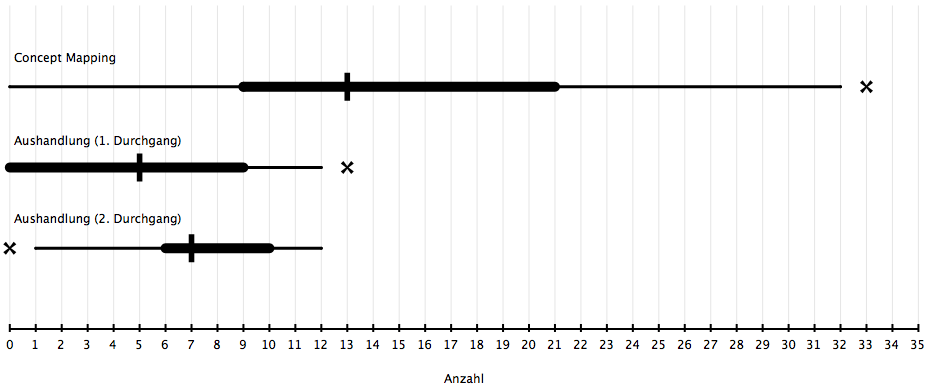
\includegraphics[width=15cm]{img/Evaluierung/elementUsageConnectorsOverview.png}
	\caption{Anzahl der verwendeten Verbindungen -- Übersicht}
	\label{fig:img_Evaluierung_elementUsageConnectorsOverview}
\end{figure}

Eine ähnliche Verteilung wie im Falle der Elemente ergibt sich bei Betrachtung der Anzahl der Verbindungen (siehe Abbildung \ref{fig:img_Evaluierung_elementUsageConnectorsOverview}). Auffällig ist jedoch die gegenüber Durchgang 2 des Aushandlungsblocks geringere Anzahl von Verbindungen in Durchgang 1 während sich die Anzahl der Blöcke zwischen den beiden Modellierungsdurchgängen umgekehrt verhält. Wie in der Überprüfung der Hypothese \ref{hyp:verbinder} in Abschnitt \ref{sub:herstellung_von_verbindern} bestätigt, ist dieses Phänomen auf die Fehlfunktionen und Instabilität der ursprünglichen Funktion zur Herstellung von Verbindungen zurückzuführen, die in Durchgang 1 ausschließlich zur Verfügung stand, während in Durchgang 2 (und auch im Block „Concept Mapping“) bereits die zusätzliche Funktion zur Verbindungsherstellung verfügbar war.

% subsubsection modellgröße (end)

\subsubsection{Vernetzungsgrad} % (fold)
\label{ssub:vernetzungsgrad}

Der Vernetzungsgrad der Modelle („Connectedness“) wurde bereits zur Überprüfung der Hypothese \ref{hyp:verbinder} in Abschnitt \ref{sub:herstellung_von_verbindern} betrachtet, ist jedoch eine Eigenschaft der erstellten Modelle an sich und wird hier deshalb nochmals als deskriptiver Parameter beschrieben.

\begin{figure}[htbp]
	\centering
		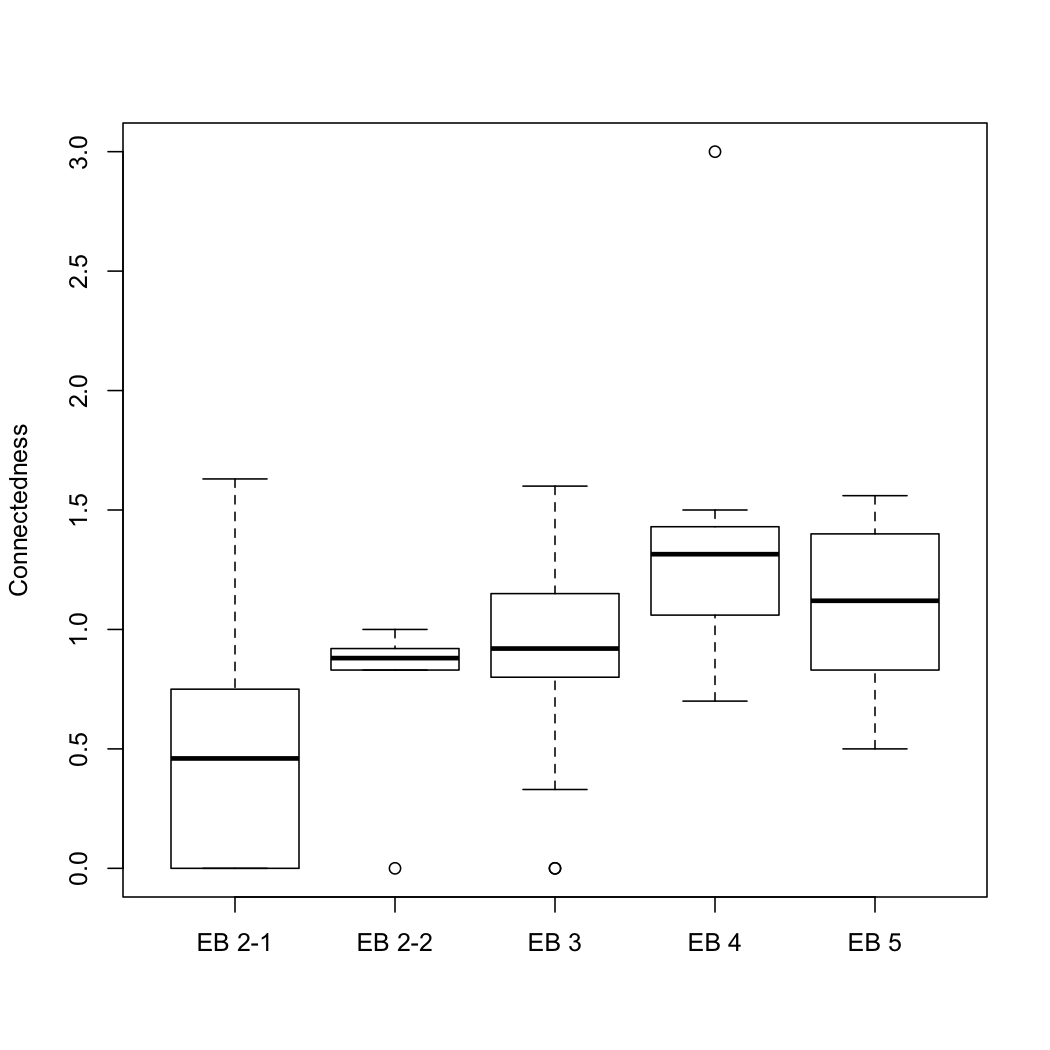
\includegraphics[width=10cm]{img/Evaluierung/connectednessOverviewAll.png}
	\caption{Vernetzungsgrad (Verbindungen / Blöcke) -- Übersicht}
	\label{fig:img_Evaluierung_connectednessOverviewAll}
\end{figure}

Abbildung \ref{fig:img_Evaluierung_connectednessOverviewAll} zeigt die Verteilung des Verhältnisses der Anzahl von Verbindungen und Blöcken in den Evaluierungsblöcken 2 bis 5. Zu erkennen ist der oben und in Abschnitt \ref{sub:herstellung_von_verbindern} bereits beschriebene geringere Vernetzungsgrad im ersten Durchgang von Evaluierungsblock 2 der auf die Instabilität und schwierige Verwendbarkeit der ursprünglichen Funktion zur Herstellung von Verbindungen zurückzuführen ist.

Seit der Verfügbarkeit der neuen Funktion zur Herstellung von Verbindungen (also im zweiten Teil von Block 2 sowie in den Blöcken 3, 4 und 5) liegt der Vernetzungsgrad im Mittel immer um oder höher 1, wobei in den letzten Blöcken (4 und 5) tendenziell noch höhere Vernetzungsgrade auftreten (Bock 4 im Mittel $1.384$ - $SD=0.617$, Block 5 im Mittel $1.101$ - $SD=0.337$). Im Falle von Block 4 kann dies teilweise auf die Aufgabenstellungen zurückgeführt werden, die zum Teil starken Fokus auf die Repräsentation von Beziehungen legte (maximaler Vernetzungsgrad in einem Durchgang: $24/8=3$). Bei beiden Blöcken wurden außerdem weitere Stabilisierungsmaßnahmen in der Interaktions-Erkennungsleistung des Systems vorgenommen, weshalb der gestiegene Vernetzungsgrad zum Teil auch auf die einfachere Herstellbarkeit von Verbindungen zurückgeführt werden kann (siehe wiederum \ref{sub:herstellung_von_verbindern}).

% subsubsection  (end)
% subsection m_durchführung (end)
% section untersuchungsdesign (end)

\section{Ergebnisse} % (fold)
\label{sec:m_ergebnisse}

In diesem Abschnitt werden die Ergebnisse der Untersuchung gegliedert nach den oben formulierten Hypothesen dargestellt. Zu jeder Hypothese wird die Auswertung der empirischen Daten dargestellt, die Bedeutung der empirischen Belege für die Prüfung der jeweiligen Hypothese diskutiert und letztendlich das Ergebnis zusammenfassend dargestellt.  

\subsection{Keine semantische Einschränkung der Externalisierung} % (fold)
\label{sub:keine_semantische_einschränkung_der_externalisierung}

Gegenstand der hier beschriebenen Untersuchung Hypothese \ref{hyp:keine_einschränkung} („Das Werkzeug schränkt Benutzer semantisch nicht bei der Externalisierung ihrer mentalen Modelle ein.“). Als Grundlage dieser Untersuchung dienen die Ergebnisse der Evaluierungsblöcke 2 bis 5, da in diesen die den einzelnen Modellelementen zugewiesene Semantik explizit untersucht wurde. Die Daten hinsichtlich der empfundenen Einschränkung bei der Modellbildung stammen aus der Befragung, die im Rahmen des Evaluierungsblocks 4 durchgeführt wurde. Zusätzlich wurde das Videomaterial aller fünf Evaluierungsblöcke zur Auswertung herangezogen.

\subsubsection{Auswertung} % (fold)

Die „Nicht-Einschränkung“ der Benutzer bei der Externalisierung kann wie in Abschnitt \ref{ssub:keine_semantische_einschränkung_der_externalisierung} beschrieben anhand des Modellierungsverhaltens der Benutzer beurteilt werden. Von Interesse ist hier die Zuweisung von Bedeutung (also semantischer Information) zu den (semantisch nicht vorbelegten) Modellierungselementen. Davon stehen grundsätzlich drei Arten von Blöcken („rot“, „gelb“, „blau“) sowie drei Arten von Verbindern („ungerichtet“, „gerichtet“, „bidirektional“). Erhoben wurde, wie viele Elemente im Verlauf der Modellierung mit Bedeutung belegt wurden, ob die Teilnehmenden mehr als die zur Verfügung stehenden Elemente benötigt hätten und ob ein Element im Modellierungsverlauf mit mehr als einer Bedeutung belegt wurde. 

Zu beachten ist hier, das die Bedeutungsbelegung immer Ergebnis eines Aushandlungsprozesses zwischen mindestens zwei Beteiligten ist. Aus dieser Teiluntersuchung kann also kein Rückschluss auf die individuell empfundene Einschränkung der Externalisierung getroffen werden. Nachdem der Prozess der Bedeutungsfestlegung aber inhärenter Bestandteil der kooperativen Modellbildung ist und die Zielsetzung derselben die Herstellung eines gemeinsamen Verständnisses ist, ist dies im Falle einer tatsächlich kooperativ vorgenommenen Festlegung der Bedeutung nicht als Einschränkung zu sehen. Eine individuell als einschränkend wahrgenommene Situation kann vielmehr dann auftreten, wenn die Bedeutungsfestlegung nicht kooperativ durchgeführt wurde, sondern die Bedeutungen von einem Teilnehmenden vorgegeben wurde. Diese Fälle sind in der folgenden Tabelle separat ausgeführt. Die individuell empfundene Einschränkung wurde außerdem im zweiten Teil der hier beschriebenen Untersuchung mittels einem auf dem \gls{PMS} basierenden Fragebogen sowie einer Auswertung der offenen Fragen zur Eignung des Werkzeugs zur Modellbildung erhoben. 

In Tabelle \ref{tab:anzahl_bedeutungstragende_elemente} ist für jeden Evaluierungsblock ausgeführt, in wie vielen Fällen eine bestimmte Anzahl von Blöcken mit Bedeutung belegt wurde und wie viele Arten von Verbindern benutzt wurden. Unterschiedliche Bedeutungen auf unterschiedlichen Modellebenen (also in eingebetteten Teilmodellen) wurden ohne separaten Unterscheidung mitgezählt.

\begin{table}[htbp]
	\centering
	\caption{Anzahl der bedeutungstragenden Elemente je Modell}
\begin{tabular}{| c || c | c | c | c || c | c | c | c |}
  \hline
   EB & 1 E. & 2 E. & 3 E. & 4+ E. & 1 V. & 2 V. & 3 V. & 4+ V. \\ \hline
   2 - 1 & 0 & 2 &  9 & 0 &  4 &  1 & 0 & 0 \\ 
   2 - 2 & 1 & 0 &  8 & 0 &  6 &  1 & 0 & 1 \\ 
   3     & 0 & 3 & 14 & 0 &  6 &  4 & 0 & 6 \\ 
   4     & 0 & 2 &  7 & 2 &  3 &  4 & 2 & 1 \\ 
   5     & 0 & 1 &  7 & 3 & 11 &  0 & 0 & 0 \\ \hline
   Ges.  & 1 & 8 & 45 & 5 & 30 & 10 & 2 & 8 \\ \hline
\end{tabular} \\
\footnotesize EB \ldots Evaluierungsblock, x E.\ldots x Elemente mit Bedeutung belegt, x V. \ldots x Arten von Verbindungen verwendet
	\label{tab:anzahl_bedeutungstragende_elemente}
\end{table}
 
In jenen beiden Fällen in Evaluierungsblock 4 und den drei Fällen in Evaluierungsblock 5, in denen 4 oder mehr bedeutungstragende Elemente verwendet wurden, wurden zweimal 4, und je einmal 6, 7 und 9 Elementtypen festgelegt. Beide Modelle enthielten jedoch ineinander verschachtelte Teilmodelle, von denen keines mehr als drei Typen beinhaltete. Jene Fälle, in denen 4 oder mehr verschiedene Arten von Verbindern verwendet wurden, kamen durch den Einsatz benannter Verbinder zustande, mittels derer die Bedeutung der Verbindungen beliebig differenziert werden kann.

Im zweiten Teil der Untersuchung zu dieser Hypothese wurden qualitativ einerseits die expliziten Aussagen der Teilnehmenden ($n_{ges}=139$) hinsichtlich einer eventuellen einschränkenden Wirkung des Werkzeugs gesammelt, andererseits wurden die Videoaufnahmen der Werkzeuganwendungen diesbezüglich ausgewertet. Folgende Punkte mit einschränkender Wirkung konnten hier identifiziert werden (in Klammern jeweils die Quellen sowie die Anzahl des Auftretens der jeweiligen Aussage):
\begin{itemize}
	\item Unterschiedliche Farben von Verbindern wären wünschenswert (Befragung in Block 4, $n=2$)
	\item Drei unterschiedliche Elementtypen sind zu wenig (verbales Feedback von Personen mit praktischen Prozessmodellierungskenntnissen\footnote{Nach diesen Kenntnissen wurde im Rahmen einer Selbsteinschätzung explizit gefragt} in den Blöcken 2 und 4 sowie in nicht formal dokumentieren Modellierungssitzungen mit Prozessmodellierungsexperten\footnote{jeweils nach Eigendeklaration bzw. aus dem professionellen Umfeld der Personen geschlossen} im Rahmen von Demonstrationen auf mehreren Konferenzen, $n=7$)
	\item Dezidierte Elemente zur Modellierung von Verzweigungen und Parallelisierungen im Kontrollfluss wären wünschenswert (verbales Feedback von Personen mit Prozessmodellierungskenntnissen in den Blöcken 2 und 4 sowie in nicht formal dokumentieren Modellierungssitzungen mit Prozessmodellierungsexperten im Rahmen von Demonstrationen auf mehreren Konferenzen, $n=5$)
	\item Selbst festlegbare Formen, Farben und/oder Größen von Modellelementen wären wünschenswert (verbales Feedback von Personen in Block 4 sowie in nicht formal dokumentieren Modellierungssitzungen mit  Strukturaufstellungsexperten\footnote{das Werkzeug scheint sich zur Unterstützung von Strukturaufstellungen \citep{Sparrer02} zu eignen, dies wurde jedoch im Rahmen dieser Arbeit weder als Anwendungsfall vorgesehen, noch formal getestet} im Rahmen von Demonstrationen auf mehreren Konferenzen, $n=3$)
\end{itemize}

Explizite Aussagen zu einer dezidiert „nicht-einschränkenden“ Wirkung bzw. der semantischen Offenheit des Werkzeugs konnten nur in Fällen identifiziert werden, in denen explizit nach diesem Aspekt gefragt wurde. In diesen Fällen wurde der Umfang der Ausdrucksmöglichkeiten durchwegs als ausreichend erachtet. Personen ohne Vorkenntnisse in der Prozessmodellierung empfanden die Anzahl der zur Verfügung stehenden Elemente im Allgemeinen als ausreichend, jene Fälle in denen dies nicht der Fall war, sind oben dokumentiert.

Lediglich in einem\footnote{in Evaluierungsblock 3} der dokumentierten Fälle ($n=66$) waren die Teilnehmenden mit der eigenständigen Wahl der Bedeutung der Elementtypen überfordert und begannen nicht eigenständig zu modellieren. Erst nach einer teilweisen bzw. beispielhaften Vorgabe von 2 Elementtypen durch den Untersuchungsleiter konnten die Teilnehmenden die Modellierung selbständig fortführen. 

Vergleichend ist festzustellen, dass beim Einsatz der Werkzeugs „CMapTools“, das die Anzahl der Elementtypen nicht einschränkt, in Evaluierungsblock 5 ($n=12$) zwischen 1 und 8 Elementtypen verwendet wurden, wobei der Median bei 3 liegt. In je einem Fall wurden 1, 7 und 8 Elementtypen verwendet, in zwei Fällen wurden 3 Elementtypen eingesetzt, in drei Fällen kamen 4 Typen und in vier Fällen 2 Elementtypen zum Einsatz.

\subsubsection{Diskussion} % (fold)

Betrachtet man die Ergebnisse der quantitativen Auswertung der Einsätze des Werkzeugs in den Evaluierungsblöcken 2 bis 5, so scheint die gegebene Ausdrucksstärke für die Modellierung weitgehend ausreichend zu sein. Dieser Eindruck relativiert sich bei einer vergleichenden Betrachtung mit einem computerbasierten, semantisch vollständig offenen Werkzeug sowie bei Betrachtung der qualitativen Auswertung der Benutzeraussagen sowie der Videoaufnahmen. 

In der vergleichend durchgeführten Studie in Evaluierungsblock 5 zeigt sich, dass bei keiner Einschränkung der Anzahl der Modellelementtypen in mehr als der Hälfte der Fälle mehr als die im hier betrachteten Werkzeug zur Verfügung stehenden drei Elementtypen verwendet werden. Dies scheint darauf hinzudeuten, dass sich die Teilnehmenden an der beschränkten Anzahl der zur Verfügung stehenden Elemente orientieren, auch wenn dies -- wie aus den Aussagen der Teilnehmenden bei der ex-post-Befragung ersichtlich -- bis auf einige Ausnahmen nicht als Einschränkung wahrgenommen wird.

Aus den qualitativen Rückmeldungen zur Modellierung zeigt sich außerdem, dass Personen, die in ihrer täglichen Arbeit aktiv mit Prozessmodellierung beschäftigt sind, bei Aufgabenstellungen, die aufgrund ihrer Fragestellung zu Ablaufbeschreibungen führen, eher die Verwendung von mehr als drei Elementtypen bevorzugen würden. Personen, denen Prozessmodellierung fremd ist oder deren Erfahrung damit sich auf eine einmalige, länger zurückliegende Ausbildung beschränkt, konnten ihre Modelle zu ablauforientierten Fragestellungen ohne Ausnahme mit maximal drei Elementtypen abbilden. Bei nicht ablauforientierten Fragestellungen ist diese Unterscheidung nicht zu beobachten.

In Einzelfällen wurden außerdem weitere Wünsche zur Steigerung der Ausdrucksmöglichkeiten im Modell geäußert. Neben dem Wunsch nach unterschiedlich einfärbbaren Verbindungen zwischen Elementen wurde vor allem der Wunsch nach der Verwendung beliebiger Gegenstände als Modellelemente mehrfach geäußert, was das Einbringen von Repräsentation aus der alltäglichen Arbeitspraxis anstelle der abstrakten Modellelemente erlauben würde.

Unter Berücksichtigung dieser Einschränkungen kann die hier betrachtete Hypothese mit Vorbehalten bestätigt werden. Tatsächlich scheint das Werkzeug bis auf wenige Ausnahmen nicht als semantisch einschränkend wahrgenommen zu werden, die Ergebnisse der vergleichenden Studie weisen aber auf eine einschränkende Wirkung durch die auf drei beschränkte Anzahl von Elementtypen hin.

\subsubsection{Ergebnis} % (fold)

\textbf{Die Hypothese \ref{hyp:keine_einschränkung} kann in der Untersuchung mit Vorbehalten angenommen werden.} Die Verwendung des Werkzeugs zur Modellierung scheint (bis auf wenige Ausnahmen) nicht als semantisch einschränkend wahrgenommen zu werden. Die vergleichende Studie aus Evaluierungsblock 5 deutet allerdings auf eine einschränkende Wirkung durch die auf drei beschränkte Anzahl von Elementtypen hin.

% subsection keine_semantische_einschränkung_der_externalisierung (end)

\subsection{Repräsentation beliebig umfangreicher Modelle} % (fold)
\label{sub:repräsentation_beliebig_komplexer_modelle}

Gegenstand der hier beschriebenen Untersuchung Hypothese \ref{hyp:beliebige_komplexität} („Das Werkzeug ermöglicht die Repräsentation beliebig umfangreicher Modelle.“). Als Grundlage dieser Untersuchung dienen die Ergebnisse der Modellbildung in Evaluierungsblock 3 und 5 sowie die Befragungen in den Evaluierungsblöcken 1 bis 5.

\subsubsection{Auswertung} % (fold)

Von Interesse ist bei der Prüfung dieser Hypothese der Vergleich des Umfangs von Modellen, die mit dem hier vorgestellten Werkzeug erstellt wurden, mit Modellen, die mit einem bezogen auf die Größe der Arbeitsfläche unbeschränkten Werkzeug erstellt wurden. Diese vergleichende Studie wurde im Rahmen der Untersuchungen in Block 5 durchgeführt. Als Metrik zum Vergleich der Modellgrößen wurde die Anzahl der Modellelemente verwendet. Abbildung \ref{fig:img_Evaluierung_ElementeConceptMapping2} zeigt eine Gegenüberstellung der Modellgrößen bei Verwendung der „CMapTools“ als die Größe nicht beschränkendes Werkzeug und dem hier vorgestellten System\footnote{In allen Boxplots gilt folgende Notation: 
\begin{itemize}
	\item breite horizontale Linie: Bereich zwischen 25\%- und 75\%-Quantil
	\item breite vertikale Linie: Median
	\item linke schmale Linie: Bereich zwischen 2,5\%- und 25\%-Quantil
	\item rechte schmale Linie: Bereich zwischen 75\%- und 97,5\%-Quantil
	\item Kreuze: Ausreißer (außerhalb 2,5\%- und 97,5\%-Quantil)
\end{itemize}
}.

\begin{figure}[htbp]
	\centering
		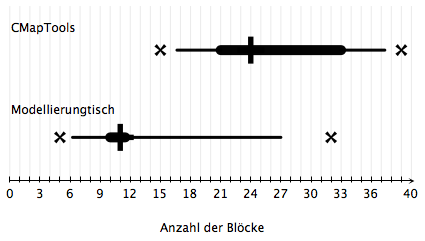
\includegraphics[width=10cm]{img/Evaluierung/ElementeConceptMapping2.png}
	\caption{Gegenüberstellung der Modellgrößen in Evaluierungsblock 5}
	\label{fig:img_Evaluierung_ElementeConceptMapping2}
\end{figure}

Die Betrachtung der Ergebnisse zeigt, dass die Modelle, die mittels der „CMapTools“ erstellt wurden ($M=25.92, SD=7.04, n=12$), signifikant umfangreicher waren (einseitiger Wilcoxon-Test für ungepaarte Stichproben: $W=8, p<0.001$\footnote{Der Wilcoxon-Test muss angewandt werden, da die zweite Stichprobe nicht normalverteilt ist (Shaprio-Wilk-Test: $W_{CMap} = 0.9136, p_{CMap} = 0.2372$, $W_{Tisch} = 0.5786, p_{Tisch} < 0.005$)}), als jene Modelle, die mittels dem hier vorgestellten System erstellt wurden ($M=12.18, SD=6.84, n=11$).

In den Evaluierungsblöcken 3 und 5 wurden insgesamt 30 Modellierungsdurchgänge durchgeführt, deren Ergebnis aufgrund der Aufgabenstellung bei detaillierte Modellierung mehr als 15 Modellierungselement enthalten müsste (siehe vergleichende Ergebnisse aus Block 5). In insgesamt 7 Fällen wurden mehr als 15 Elemente verwendet ($15<x<=20: 1, 20<x<=25: 2, 25<x<=30: 2, x>30: 2$), der Median der Anzahl der Elemente liegt bei 11 ($M=14.68, SD=7.90, n=29$). Die Möglichkeit der Einbettung von Teilmodellen wurde insgesamt in 8 Modellierungsdurchgängen genutzt, davon war in drei Fällen die Gesamtanzahl der Elemente geringer als 15 (womit eine rein semantische Strukturierung vorliegt und keine Steigerung der Modellumfangs vorgenommen wurde).

Neben der vergleichenden Studie wurde in allen Evaluierungsblöcken der subjektive Eindruck der Teilnehmenden nach einer etwaig einschränkenden Wirkung hinsichtlich des Umfangs der Modelle gefragt ($n_{ges}=139$). Insgesamt 43 Teilnehmende empfanden die Modellierungsoberfläche als zu klein um die gewünschten Sachverhalte abzubilden. Von insgesamt 9 Teilnehmenden wurde explizit der Wunsch nach kleineren Elementen geäußert, um umfangreichere Modelle abbilden zu können. Von 23 Teilnehmenden wurde die Visualisierung der Verbindungen kritisiert („unübersichtlich“, „nur eine Verbindung zwischen zwei Blöcken möglich“), was dazu geführt hätte, dass die Modelle nicht wie ursprünglich intendiert aussähen.

\subsubsection{Diskussion} % (fold)

Sowohl die quantitativen Ergebnisse auf Evaluierungsblock 5 als auch die qualitativen Ergebnisse weisen darauf hin, dass die physische Realisierung der Modells, die mit eine Beschränkung der Modellierungsoberfläche einher geht, die Abbildung beliebig umfangreicher Modelle nicht erlaubt.

Bei der Gegenüberstellung des quantitativen Teils der Studie mit den qualitativen Aussagen der Teilnehmenden fällt auf, dass -- wie bereits bei der Diskussion der Hypothese \ref{hyp:keine_einschränkung} in Abschnitt \ref{sub:keine_semantische_einschränkung_der_externalisierung} -- die subjektive Wahrnehmung der Einschränkung weniger stark ausgeprägt ist als die vermutete tatsächliche Einschränkung, auf die aufgrund der quantitativen Daten geschlossen werden kann. Tatsächlich ist jedoch der Anteil der Teilnehmer, die das Modell nicht so umfangreich wie intendiert abbilden konnten, höher als jener die sich in der semantischen Ausdrucksstärke eingeschränkt fühlten.

Aus den qualitativen Aussagen ist zu erkennen, das der vorrangige Grund der Beschränkung des Modellumfangs die eingeschränkte Größe der Modellierungsoberfläche ist. Die Möglichkeit zur Einbettung von Teilmodellen zur Steigerung des Umfangs wurde nur in einem Sechstel der Fälle verwendet, was darauf hindeutet, dass diese Funktion keinen Ersatz für eine unbeschränkt große Modellierungsoberfläche (auf einer Abstraktionsebene) darstellt.

Insgesamt kann aufgrund der Ergebnisse der Untersuchung die Hypothese \ref{hyp:beliebige_komplexität} nicht bestätigt werden.

\subsubsection{Ergebnis} % (fold)

\textbf{Die Hypothese \ref{hyp:beliebige_komplexität} kann in der Untersuchung nicht bestätigt werden.} Modelle, die mit dem hier vorgestellten Werkzeug erstellt wurden, weisen bei identischer Aufgabenstellung einen signifikant geringeren Umfang auf als Modelle, die mit einem Werkzeug mit nicht beschränkter Arbeitsfläche erstellt wurden. Auch das qualitative Feedback der Benutzer deutet darauf hin, dass eine vollständige Abbildung eines Modells (und damit die Erstellung eines Modells mit größerem Umfang) nicht bzw. nur umständlich möglich ist.

% subsection repräsentation_beliebig_komplexer_modelle (end)

% subsection abstimmung_individueller_modelle (end)

\subsection{Reflexion des Modellierungsverlaufs} % (fold)
\label{sub:reflexion_des_modellierungsverlaufs}

Gegenstand der hier beschriebenen Untersuchung ist Hypothese \ref{hyp:historie} („Die Reflexion des Modellierungsverlaufs ermöglicht das Verständnis der dem Modell abgebildeten Inhalte.“). Als Grundlage dieser Untersuchung dienen die Ergebnisse der Evaluierungsblöcke 4 und 5, da die Erfassung und Persistierung der gesamten Modellierungshistorie erst in diesen Blöcken zuverlässig arbeitete.

\subsubsection{Auswertung} 
 
Zur Prüfung dieser Hypothese wurden die Modelle aus den Evaluierungsblöcken 4 (Einsatz im Unternehmenskontext) und 5 (Concept Mapping 2 -- lediglich jene Anwendungen, die mit dem Modellierungstisch durchgeführt wurden) herangezogen. Die Interpretation der erstellten Modelle wurde jeweils von einer Person vorgenommen, die an der eigentlichen Modellierung nicht beteiligt war. Die Beurteilung der Korrektheit und Vollständigkeit der Interpretation hinsichtlich der von den Modellierungsteilnehmern ausgedrückten Inhalte erfolgte durch den jeweiligen Untersuchungsleiter, da die Modellierer selbst nicht mehr zur Verfügung standen.

Interpretiert wurde jeweils einerseits das eigentliche Endergebnis und andererseits das Endergebnis inklusive aller erfassten Zwischenzustände des Modells während der Modellentstehung. Beide Interpretationen wurden gegenübergestellt und hinsichtlich ihrer Korrektheit und Vollständigkeit auf einer vierteiligen Likert-Skala beurteilt („korrekt“ -- „eher korrekt“ -- „eher nicht korrekt“ -- „nicht korrekt“). Zusätzlich wurden qualitativ etwaige Auffälligkeiten bei abweichenden Interpretationen erhoben.

Im Falle des Evaluierungsblocks 4 wurden 10 Modelle interpretiert. Bei der Interpretation ergab sich die in Tabelle \ref{tab:interpretation_block4} dargestellte Verteilung.

\begin{table}[htbp]
	\centering
	\caption{Korrektheit der Modellinterpretation in Evaluierungsblock 4}
\begin{tabular}{| c || c | c | c | c |}
  \hline
   & korrekt & eher korrekt & eher nicht korrekt & nicht korrekt \\ \hline
   nur Ergebnis   & 0 & 3 & 5 & 2 \\ 
   inkl. Historie & 0 & 8 & 2 & 0 \\ \hline
\end{tabular} \\
	\label{tab:interpretation_block4}
\end{table}

Im Falle des Evaluierungsblocks 5 wurden 11 Modelle interpretiert. Bei der Interpretation ergab sich die in Tabelle \ref{tab:interpretation_block5} dargestellte Verteilung.

\begin{table}[htbp]
	\centering
	\caption{Korrektheit der Modellinterpretation in Evaluierungsblock 5}
\begin{tabular}{| c || c | c | c | c |}
  \hline
   & korrekt & eher korrekt & eher nicht korrekt & nicht korrekt \\ \hline
   nur Ergebnis   & 6 & 4 & 1 & 0 \\ 
   inkl. Historie & 6 & 4 & 1 & 0 \\ \hline
\end{tabular} \\
	\label{tab:interpretation_block5}
\end{table}

Für die Untersuchung des Unterschiedes zwischen den beiden Interpretationsarten wurde der Wilcoxon-Test herangezogen. Dies war notwendig, da der Shapiro-Wilk-Test zeigte, dass beide Stichproben nicht normalverteilt waren ($n_{Ergebnis}=21, p_{Ergebnis}=0.012, n_{Historie}=21, p_{Historie}<0.005$).

Entsprechend dieser Testergebnisse wurde ein einseitiger Wilcoxon-Test für gepaarte Stichproben durchgeführt. Dieser ergab für die Interpretationen unter Einbeziehung der Historie ($n=21, M=1.86, SD=0.655$) eine signifikant „korrektere“ Bewertung ($n=21, p=0.00537$) als für die Interpretationen auf Basis des Modellierungsergebnisses ($n=21, M=2.19, SD=0.981$).

Trennt man beide Untersuchungen auf, so ergibt sich unter Einsatz der gleichen Test-Verfahren für die Untersuchung in Evaluierungsblock 4 ein signifikant korrekteres Ergebnis ($n=10, p=0.0107$) für die Interpretation unter Einbeziehung der Historie ($n=10, M=2.2, SD=0.422$) gegenüber der Interpretation auf Basis des Modellierungsergebnisses ($n=10, M=2.90, SD=0.738$). In Evaluierungsblock sind die Verteilungen der Korrektheitsbeurteilung in beiden Interpretationsvarianten identisch ($n=11, M=1.55, SD=0.688$), so dass sich kein signifikanter Unterschied ergeben kann.

\subsubsection{Diskussion} 

Aus den Untersuchungsergebnissen ist zu erkennen, dass die Interpretation auf Basis der Modellierungshistorien signifikant besser (d.h. vollständiger und korrekter) ist als die Interpretation ausschließlich auf Basis des Modellierungsergebnisses. Vor allem ablauf-orientierte Modelle (wie in Block 4 vorherrschend) scheinen auf Basis der Modellierungshistorie besser zu interpretieren zu sein (wenn auch auf generell niedrigem Niveau -- siehe oben). Im Falle von Modellen, in denen eher konzeptuelle Strukturen abgebildet wurden (wie die Modelle in Block 5) scheint eine Interpretation generell einfacher möglich zu sein -- hier zeigt sich allerdings kein Mehrwert bei der Interpretation der Modellierungshistorie. Die hier geprüfte Hypothese kann also auf Basis der beschriebenen Untersuchung bestätigt werden.

Generell ist die eher niedrige Einschätzung von Korrektheit und Vollständigkeit bei Interpretation der Ergebnisse rein auf Basis von dokumentierten Modellen (sei es das Endergebnis oder die Historie). Diese fällt weitaus geringer aus als eine Interpretation auf Basis der ebenfalls vorliegenden Videoaufnahmen der Modellierungen (diese wurde jedoch nicht formal evaluiert und deshalb nicht in die obige Gegenüberstellung aufgenommen). Fraglich bleibt an dieser Stelle, ob die Nachvollziehbarkeit der mit dem hier vorgestellten System abgebildeten Inhalte ausschließlich auf Basis der gelegten Strukturen gegeben ist. Die kompaktere Modelldarstellung (gegenüber bildschirmbasierten Werkzeugen, siehe Abschnitt \ref{sub:repräsentation_beliebig_komplexer_modelle}) und der eher auf Diskussion denn auf Abbildung fokussierte Modellierungprozess (siehe Abschnitt \ref{sub:wirkung_auf_die_kooperation_bei_der_modellerstellung}) scheinen hier eine einschränkende Wirkung zu entfalten.

\subsubsection{Ergebnis} 

\textbf{Die Hypothese \ref{hyp:historie} kann auf Basis der Untersuchung bestätigt werden.} Die Korrektheit und Vollständigkeit der Interpretation von Modellen kann durch die Einbeziehung der Modellierungshistorie signifikant gesteigert werden, ist aber vor allem bei Modellen, die aus ablauforientierten Fragestellungen entstanden sind, als eher gering einzuschätzen. 

\subsection{Wirkung auf die Kooperation bei der Modellerstellung} % (fold)
\label{sub:wirkung_auf_die_kooperation_bei_der_modellerstellung}

Gegenstand der hier beschriebenen Untersuchung Hypothese \ref{hyp:stärkere_kooperation} („Die Verwendung des Werkzeugs führt zu stärkerer Kooperation bei der Modellerstellung als die Verwendung von bildschirm-basierten Werkzeugen.“). Als Grundlage dieser Untersuchung dienen die Videoaufnahmen sowie die Ergebnisse der Teilnehmerbefragung des Evaluierungsblocks 5.

\subsubsection{Auswertung} % (fold)

Zur Beurteilung des Ausmaßes der Kooperation lässt sich aus dem Prozess der Modellbildung heraus an der Verteilung der Modellierungszeit zwischen den Teilnehmern, den Anzahl der Initiativwechsel sowie dem Anteil von Diskussionszeit an der Gesamtmodellierungsdauer messen.

Die Zeitverteilung zwischen den Teilnehmern betrug bei der Durchführung mittels CMapTools bei einer Gruppengröße von 2 Personen für Teilnehmer A im Schnitt 19 Minuten 21 Sekunden ($SD=8:11, N=11$) und für Teilnehmer B im Schnitt 14 Minuten 44 Sekunden ($SD=5:54, N=11$). Setzt man diese Werte zueinander ins Verhältnis ergibt sich ein Anteil von $56.88\%$ für Teilnehmer A und $43.12\%$ für Teilnehmer B. Bei jener Anwendung, die von drei Personen durchgeführt wurde ergab sich die Verteilung 20 min - 12 min - 8 min. 

Bei der Durchführung am Modellierungstisch ergab sich bei einer Gruppengröße von 2 Personen für Teilnehmer A im Schnitt 17 Minuten und 18 Sekunden ($SD=6:59, N=9$) und für Teilnehmer B im Schnitt 13 Minuten 12 Sekunden ($SD=6:01, N=9$). Setzt man diese Werte zueinander ins Verhältnis ergibt sich ein Anteil von $57.52\%$ für Teilnehmer A und $42.48\%$ für Teilnehmer B. Bei den beiden Anwendungen, an denen drei Personen beteiligt waren, ergab sich eine Verteilung von 5 min - $2.5$ min - $2.5$ min bzw. 20 min - 10 min - 3 min. 

Der Unterschied zwischen den Anteilen im Verhältnis zur gesamten Modellierungsdauer (${t_{TN A} - t_{TN B}}/t_{ges}$\footnote{Als Teilnehmer A wird immer jener Teilnehmer bezeichnet, der den höheren Zeitanteil in der Modellierung in Anspruch nahm.}, lediglich Anwendungen mit 2 Beteiligten wurden berücksichtigt) beträgt bei der Anwendung der CMapTools im Schnitt $0.138$ ($SD=0.086, N=11$) und am Modellierungstisch im Schnitt $0.151$ ($SD=0.087, N=9$). Zwischen diesen beiden Werten kann kein signifikanter Unterschied festgestellt werden (zweiseitiger Wilcoxon-Test: $W=51, p=0.8588, N=20$\footnote{Die Durchführung des Wilcoxon-Test ist aufgrund der Nicht-Normalverteilung beider Stichproben notwendig (Shapiro-Wilk-Test: $W_{CMap} = 0.9083, p_{CMap} = 0.2032$, $W_{Tisch}= 0.9642, p_{Tisch} = 0.8408$)}).

Hinsichtlich der Wechsel der Initiative waren bei der Durchführung der Modellierung mittels CMapTools ($N=12$) 8 Fälle zu beobachten, in denen ein Teilnehmer exklusiven Zugriff auf die Eingabemedien über den gesamten Verlauf der Modellierung hatte. In 2 Fällen fanden zwei Initiativ-Wechsel statt, in jeweils 1 einem Fall fanden 4 bzw. 8 Initiativ-Wechsel statt. Bei der Durchführung der Modellierung it dem hier vorgestellten System ($N=11$) wurde in 7 Fällen simultan an der Benutzungsschnittstelle gearbeitet, es konnten keine Initiativ-Wechsel im Sinne obiger Definition festgestellt werden. In 2 Fällen wurden je 2 Wechsel der Initiative festgestellt, in zwei Fällen kam es zu keinem Initiativ-Wechsel.

Der Anteil von Diskussionszeit an der Gesamtmodellierungsdauer betrug bei der Durchführung mittels CMapTools im Schnitt $57.15\%$ ($SD=7.49\%, N=12$) und war damit signifikant niedriger (einseitiger Wilcoxon-Test: $W=120, p<0.001, N=23$) als der Diskussionsanteil bei der Arbeit am Modellierungstisch mit im Schnitt $76.08\%$ ($SD=8.84\%, N=11$).

In Evaluierungsblock 5 wurden die Teilnehmer außerdem quantitativ und qualitativ nach dem Einfluss des Werkzeugs auf die Kooperation befragt. In der quantitativen Auswertung wurden 2 Items (Abschnitt „Kollaboratives Modellieren“ in Block 5 -- siehe Anhang \ref{sub:fb_eval5}) betrachtet, deren Gegenüberstellung einen Vergleich der wahrgenommenen Wirkung der beiden eingesetzten Werkzeuge ermöglicht. Die Items lauten im einzelnen:

\begin{enumerate}
	\item Ich konnte meine persönliche Meinung und Ideen ausreichend einbringen.
	\item Das Werkzeug hat die Zusammenarbeit als Team erleichtert.
\end{enumerate}

Insgesamt wurden $n_{CMap}=25$ Teilnehmer befragt, die an der Modellierung mit den CMapTools beteiligt waren. $n_{Tisch}=24$ Teilnehmer waren an der Modellierung am hier vorgestellten System beteiligt. Die Ergebnisse sind in Tabelle \ref{tab:vergleich_kooperative_modellierung} und Abbildung \ref{fig:img_Evaluierung_kollaboration_vergleich} zusammengefasst dargestellt. Neben dem Mittelwert und der Standardabweichung wurde für jedes Item auch geprüft, ob die Einschätzung als signifikant positiv zu bezeichnen ist. Dazu wurde ein einseitiger Wilcoxon-Test für die Stichprobe gegenüber dem Skalenmittelwert 4 durchgeführt \footnote{Der Wilcoxon-Test muss angewandt werden, da die Stichprobe in allen vier Fällen nicht normalverteilt ist (Shapiro-Wilk-Test: $W_{1C}=0.680, p{1C}<0.005$, $W_{1T}=0.716, p{1T}<0.005$, $W_{2C}=0.882, p{2C}=0.00742$, $W_{2T}=0.852, p{2T}<0.005$)}.

\begin{table}[htbp]
	\centering
	\caption{Befragung Kooperative Modellierung im Werkzeugvergleich -- Itemauswertung}

\begin{tabular}{| c || c | c || c | c |}
  \hline
   Item & M & SD & $V_{M<4}$ & $p_{M<4}$ \\ \hline
   $1_{CMap}$ & $1.52$ & $0.823$ & 0 & <0.005 \\ 
   $1_{Tisch}$ & $1.50$ & $0.659$ & 0 & <0.005 \\ \hline
   $2_{CMap}$ & $2.72$ & $1.49$ & 12 & <0.005 \\ 
   $2_{Tisch}$ & $2.33$ & $1.31$ & 3 & <0.005 \\ \hline
\end{tabular}
	\label{tab:vergleich_kooperative_modellierung}
\end{table}

\begin{figure}[htbp]
	\centering
		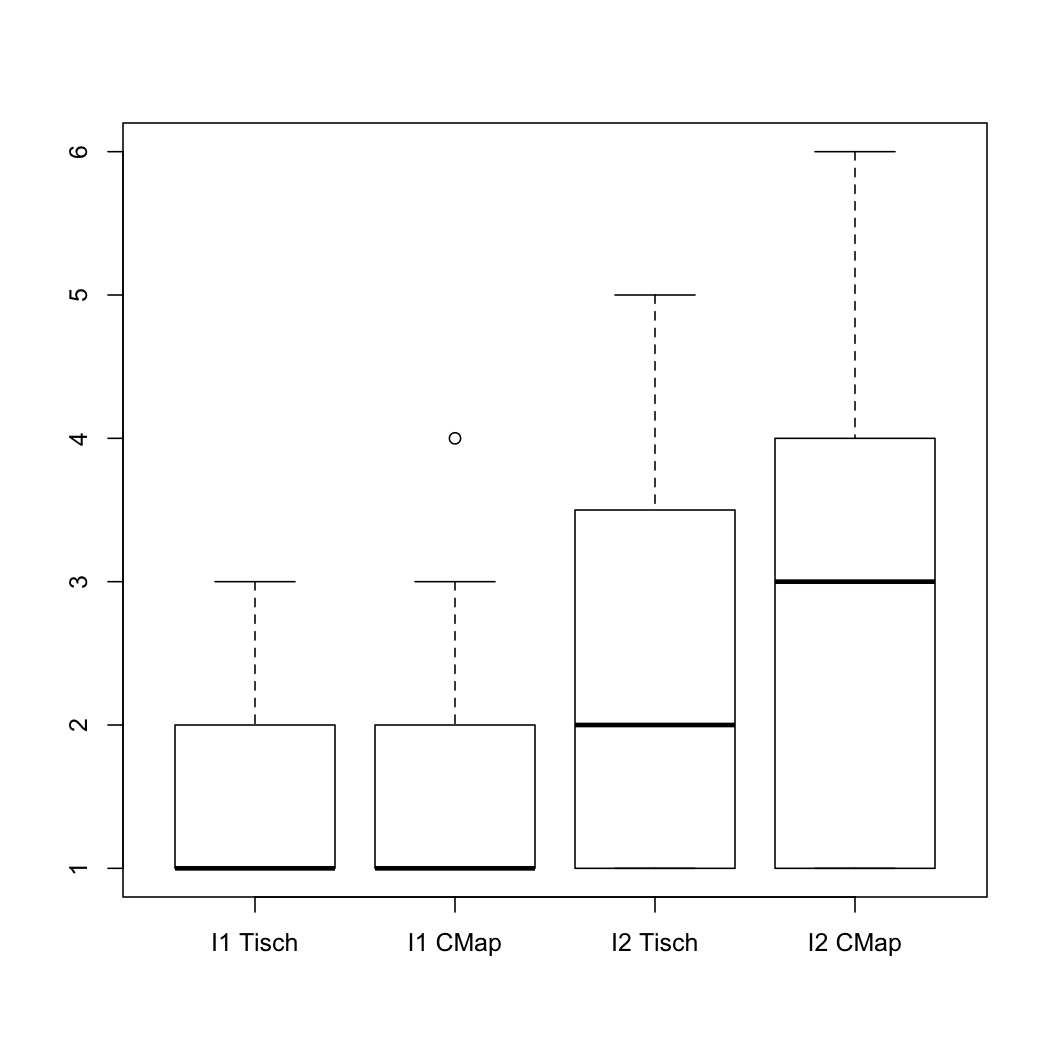
\includegraphics[height=2.5in]{img/Evaluierung/kollaboration_vergleich.png}
	\caption{Verteilung der Benutzereinschätzungen zum kooperativen Modellieren}
	\label{fig:img_Evaluierung_kollaboration_vergleich}
\end{figure}

In der Gegenüberstellung der Ergebnisse aus den beiden Teilstichproben für jedes Item zeigt sich in keinem der Fälle ein statistisch signifikanter Unterschied zwischen den beiden Stichproben (zweiseitiger Wilcoxon-Test für ungepaarte Stichproben: $W_{I1}=310, p_{I1}=0.826$, $W_{I2}=258.5, p_{I2}=0.396$).

In der qualitativen Befragung begründeten insgesamt 48 Teilnehmer (25 an den CMapTools, 23 am Modellierungstisch) ihren Eindruck (Fragestellung: „Wie würden Sie Ihre Beziehung im Team beschreiben? (Gesprächsablauf, Meinungsverschiedenheiten, gemeinsames Arbeiten mit dem Werkzeug)“). Die Ergebnisse sind im Folgenden für jeder Teilnehmergruppe inhaltlich gruppiert dargestellt.

Die Teilnehmer, die mit den CMapTools gearbeitet hatten, gaben folgende Antworten:
\begin{itemize}
	\item pos: konstruktive Arbeitsbeziehung (10x)
	\item pos: Konsens war leicht herzustellen (6x)
	\item pos: Kooperation war möglich (2x)
	\item pos: für alle zufriedenstellendes Ergebnis erreicht (2x)
	\item pos: Werkzeug ermöglicht Übersicht (1x)
	\item neutral: zu kurze Zusammenarbeit (2x)
	\item neg: ein Teilnehmer hat dominiert (2x)
\end{itemize}

Am Modellierungstisch wurden folgende Antworten gegeben:
\begin{itemize}
	\item pos: konstruktive Arbeitsbeziehung (14x) 
	\item pos: Konsens war leicht herzustellen (2x)
	\item pos: jeder konnte sich einbringen (2x) 
	\item pos: Team war okay (1x) 
	\item pos: schnelle Einigung (1x)
	\item pos: Kooperation war möglich (1x)
	\item neg: etwas planlos (2x)
\end{itemize}

\subsubsection{Diskussion} % (fold)

Die Verteilung der Modellierungsdauer zwischen den Teilnehmern als erstgenannter Indikator für funktionierende Kooperation zwischen den Teilnehmern zeigt keine signifikanten Unterschiede zwischen den beiden eingesetzten Werkzeugen. In beiden Fällen zeigt sich eine im Schnitt annähernde Gleichverteilung der Modellierungsdauer zwischen den Teilnehmern, was darauf hinweist, dass eine kooperative Modellierung sowohl mit dem Werkzeug CMapTools als auch mit dem hier vorgestellten Modellierungstisch möglich ist.

Betrachtet man jedoch die Anzahl der physischen Initiativwechsel, zeigt sich, dass die Möglichkeit des nicht-exklusiven Zugriffs auf die Benutzungsoberfläche des Modellierungtisches von den Teilnehmern genutzt wird und dazu führt, dass das die Manipulation des externalisierten Modells unmittelbar von mehr als einem Teilnehmer durchgeführt wird. Im Falle der mit der Maus und Tastatur bedienten CMapTools führt in den meisten Anwendungen ein Teilnehmer exklusiv die Manipulation des Modells durch. Durch den Wegfall des inhaltlichen „Filters“, den der manipulierende Teilnehmer potentiell bewusst oder unbewusst einführen kann, ist am Modellierungstisch eine unmittelbarere Kooperation bei der Modellerstellung möglich.

Auch die Verteilung zwischen der zur eigentlichen Modellerstellung benötigten Zeit und jener Zeit, die zum inhaltlichen Austausch über den Modellierungsgegenstand aufgewendet wird, weißt darauf hin, dass die Kooperation durch den Einsatz des Modellierungstisches im Vergleich zu den bildschirmbasierten CMapTools gestärkt wird.

Die Befragung der Benutzer zeigt jedoch keine signifikant bessere Wahrnehmung des hier vorgestellten Werkzeugs gegenüber den im Vergleich eingesetzten CMapTools. Während die Möglichkeit zur Einbringung der eigenen Sichtweise quasi identisch positiv gesehen wurde, zeigt die Einschätzung der Wirkung des Werkzeugs auf die Kooperation eine tendenziell positivere Ausprägung bei den am Modellierungstisch arbeitenden Teilnehmern. Diese Verbesserung ist jedoch nicht statistisch signifikant. Auch die qualitative Betrachtung der Benutzerantworten in den offenen Items ergibt keine wesentlichen Unterschiede in der Wahrnehmung des Werkzeugs. Lediglich hinsichtlich der negativen Auffälligkeiten wurde im Falle der CMapTools die exklusive Modellbildung durch einen Teilnehmer zweimal genannt, wohingegen die kooperative Modellbildung am Modellierungtisch von zwei Teilnehmern (die zusammengearbeitet hatten) als „etwa planlos“ bezeichnet wurde. Die Ergebnisse der Benutzerbefragung stärken die Hypothese also nicht, widersprechen ihr aber auch nicht. Insgesamt kann so die Hypothese als bestätigt angesehen werden. Zur Bestätigung aus Benutzersicht wäre eine weitere vergleichende Studie anzudenken, in der die gleichen Teilnehmer anhand verschiedener Aufgaben die Wirkung der unterschiedlichen Werkzeuge auf die Kooperation beurteilen. Die Reihenfolge der Werkzeuganwendung müsste dazu variiert werden, um Lern- bzw. Gewöhnungseffekte kompensieren zu können.

\subsubsection{Ergebnis} % (fold)

\textbf{Die Hypothese \ref{hyp:stärkere_kooperation} kann auf Basis der Untersuchung bestätigt werden.} Während die Verteilung des Zeitanteils zwischen den Modellierungsteilnehmern keinen signifikanten Unterschied zwischen den beiden verglichenen Systemen aufweist, zeigt sowohl der Vergleich der Initiativ-Wechsel als auch der Anteil an zum inhaltlichen Austausch aufgewandter Zeit einen signifikanten Vorteil hinsichtlich der Kooperationsförderung für den Modellierungstisch. Die Daten aus der Befragung der Teilnehmer stärken die Hypothese zwar nicht signifikant, zeigen aber eine leichte Tendenz zu deren Bestätigung. 

% subsection wirkung_auf_die_kooperation_bei_der_modellerstellung (end)

\subsection{Abbildung von Zusammenhängen ohne Verbinder} % (fold)
\label{sub:abbildung_von_zusammenhängen_ohne_verbinder}

Gegenstand der hier beschriebenen Untersuchung Hypothese \ref{hyp:keine_verbinder} („Zur Abbildung von Zusammenhängen ist die Verwendung von Verbindern nicht notwendig.“). Als Grundlage dieser Untersuchung dienen die Befragungen sowie die Videoaufnahmen der Evaluierungsblöcke 1 bis 5.

\subsubsection{Auswertung} % (fold)

In insgesamt 18 von den in allen 5 Evaluierungsblöcken 66 erstellten Modellen (für eine detaillierte Aufstellung siehe Abschnitt \ref{sub:repräsentation_diagrammatischer_modelle}) wurden keine Verbinder zur Darstellung von Zusammenhängen zwischen Elementen verwendet. Von diesen 18 Modellen wurden 9 Modelle (in den Evaluierungsblöcken 2 und 3) während der Modellierung von allen Beteiligten kommunikativ interpretiert. Die Teilnehmenden wurden unmittelbar nach Abschluss der Modellbildung über ihre subjektive Wahrnehmung der Übereinstimmung des Verständnisses über den abgebildeten Sachverhalt befragt. Alle Teilnehmer ($n_{ges}=21$) gaben an, subjektiv ein gemeinsames Verständnis erreicht zu haben. Diese Angaben decken sich mit den Auswertungen der Modellierungsverläufe in diesen Durchgängen, in denen in 3 von 9 Fällen während der Modellierung der Eindruck entstand, dass Teile der Modelle unterschiedlich interpretiert wurden. Diese unterschiedlichen Interpretationen wurden jedoch in allen Fällen im weiteren Verlauf der Modellierung erkannt und so abgestimmt, das ein übereinstimmendes Verständnis hergestellt werden konnte.

Jene 9 Modelle, die in Evaluierungsblock 1 erstellt wurden, wurden von Dritten interpretiert. Die Interpretation wurde dabei den ursprünglichen Modellerstellern rückgespiegelt, die wiederum zu beurteilen hatten, ob die Interpretation den ursprünglich repräsentierten Sachverhalt korrekt wiedergibt. Dies war in allen 9 Modellierungsdurchgängen der Fall (Befragung mittels einer 4-teiligen Likertskala, 6 mal „gut verstanden“, 3 mal „eher verstanden“, kein „eher nicht verstanden“ oder „nicht verstanden“). Die Abbildungen  \ref{fig:img_Evaluierung_modell_verbinder_unwichtig1} und \ref{fig:img_Evaluierung_modell_verbinder_unwichtig2} zeigen Beispiele für Modelle, in denen die korrekte Interpretation auch ohne die Darstellung von Verbindern möglich war.

\begin{figure}[htbp]
	\centering
		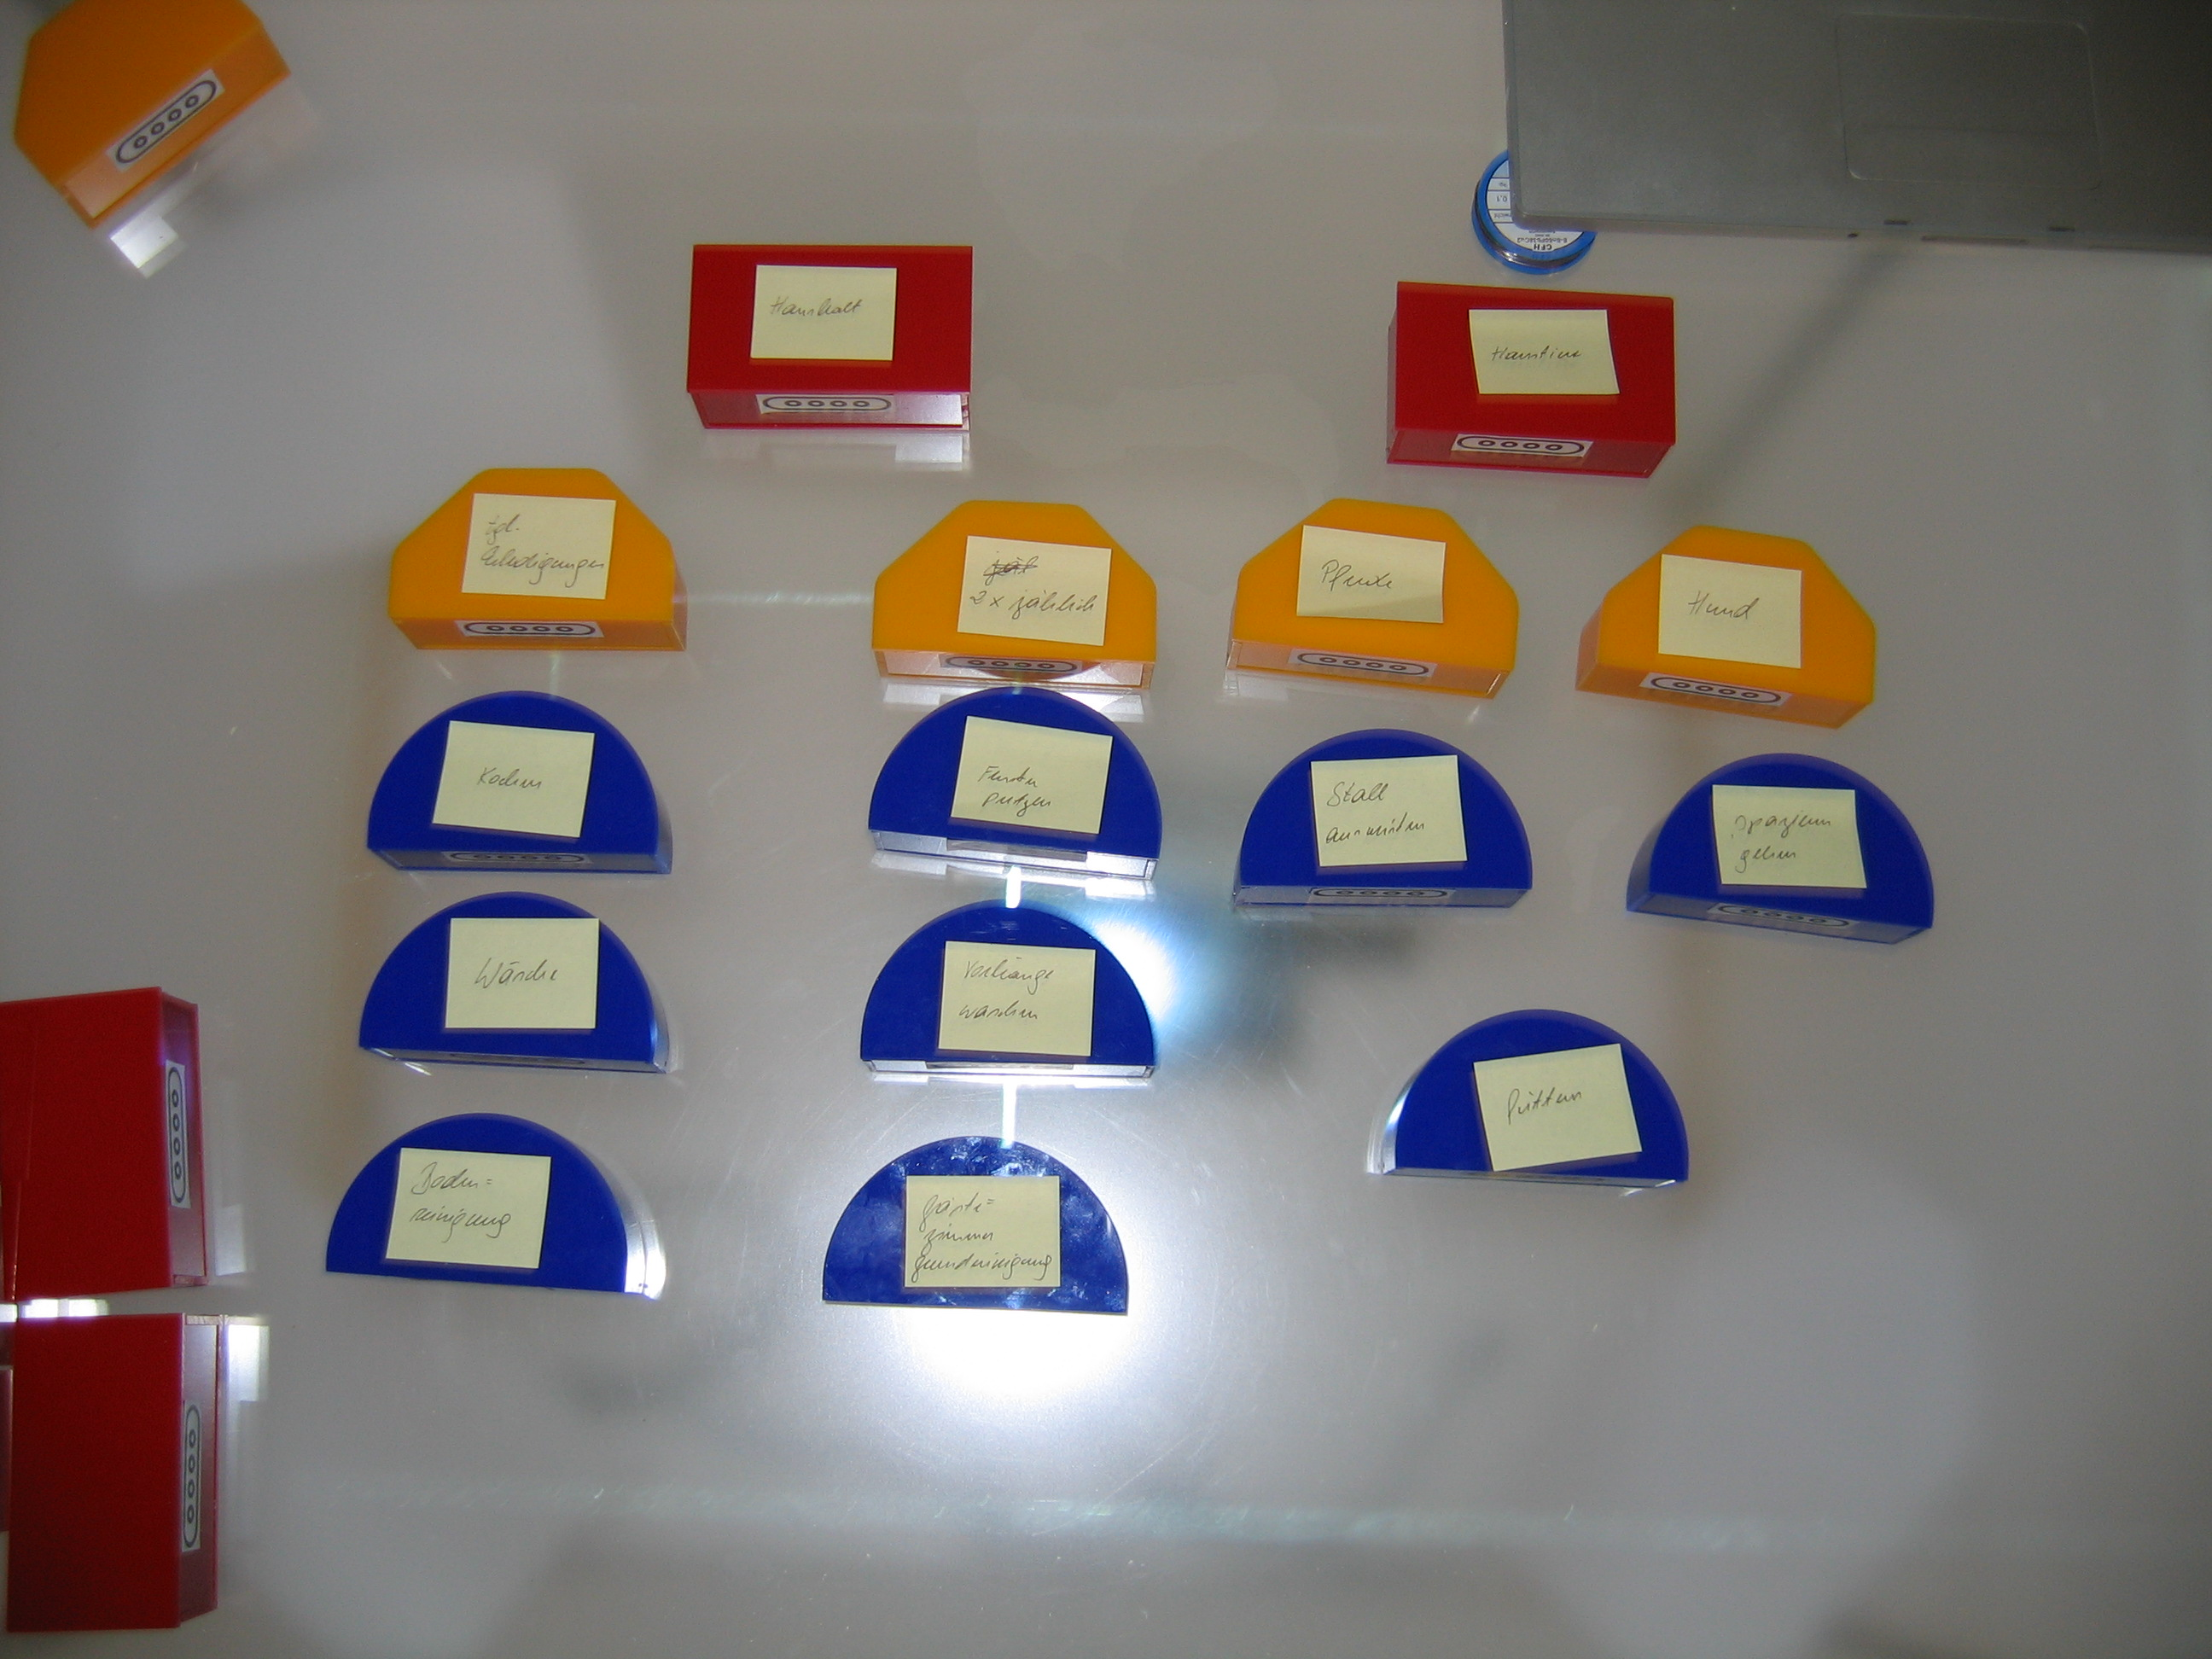
\includegraphics[width=10cm]{img/Evaluierung/modell_verbinder_unwichtig1.JPG}
	\caption{Korrekt intepretierbares Modell ohne Verbinder (hierarchisch)}
	\label{fig:img_Evaluierung_modell_verbinder_unwichtig1}
\end{figure}

\begin{figure}[htbp]
	\centering
		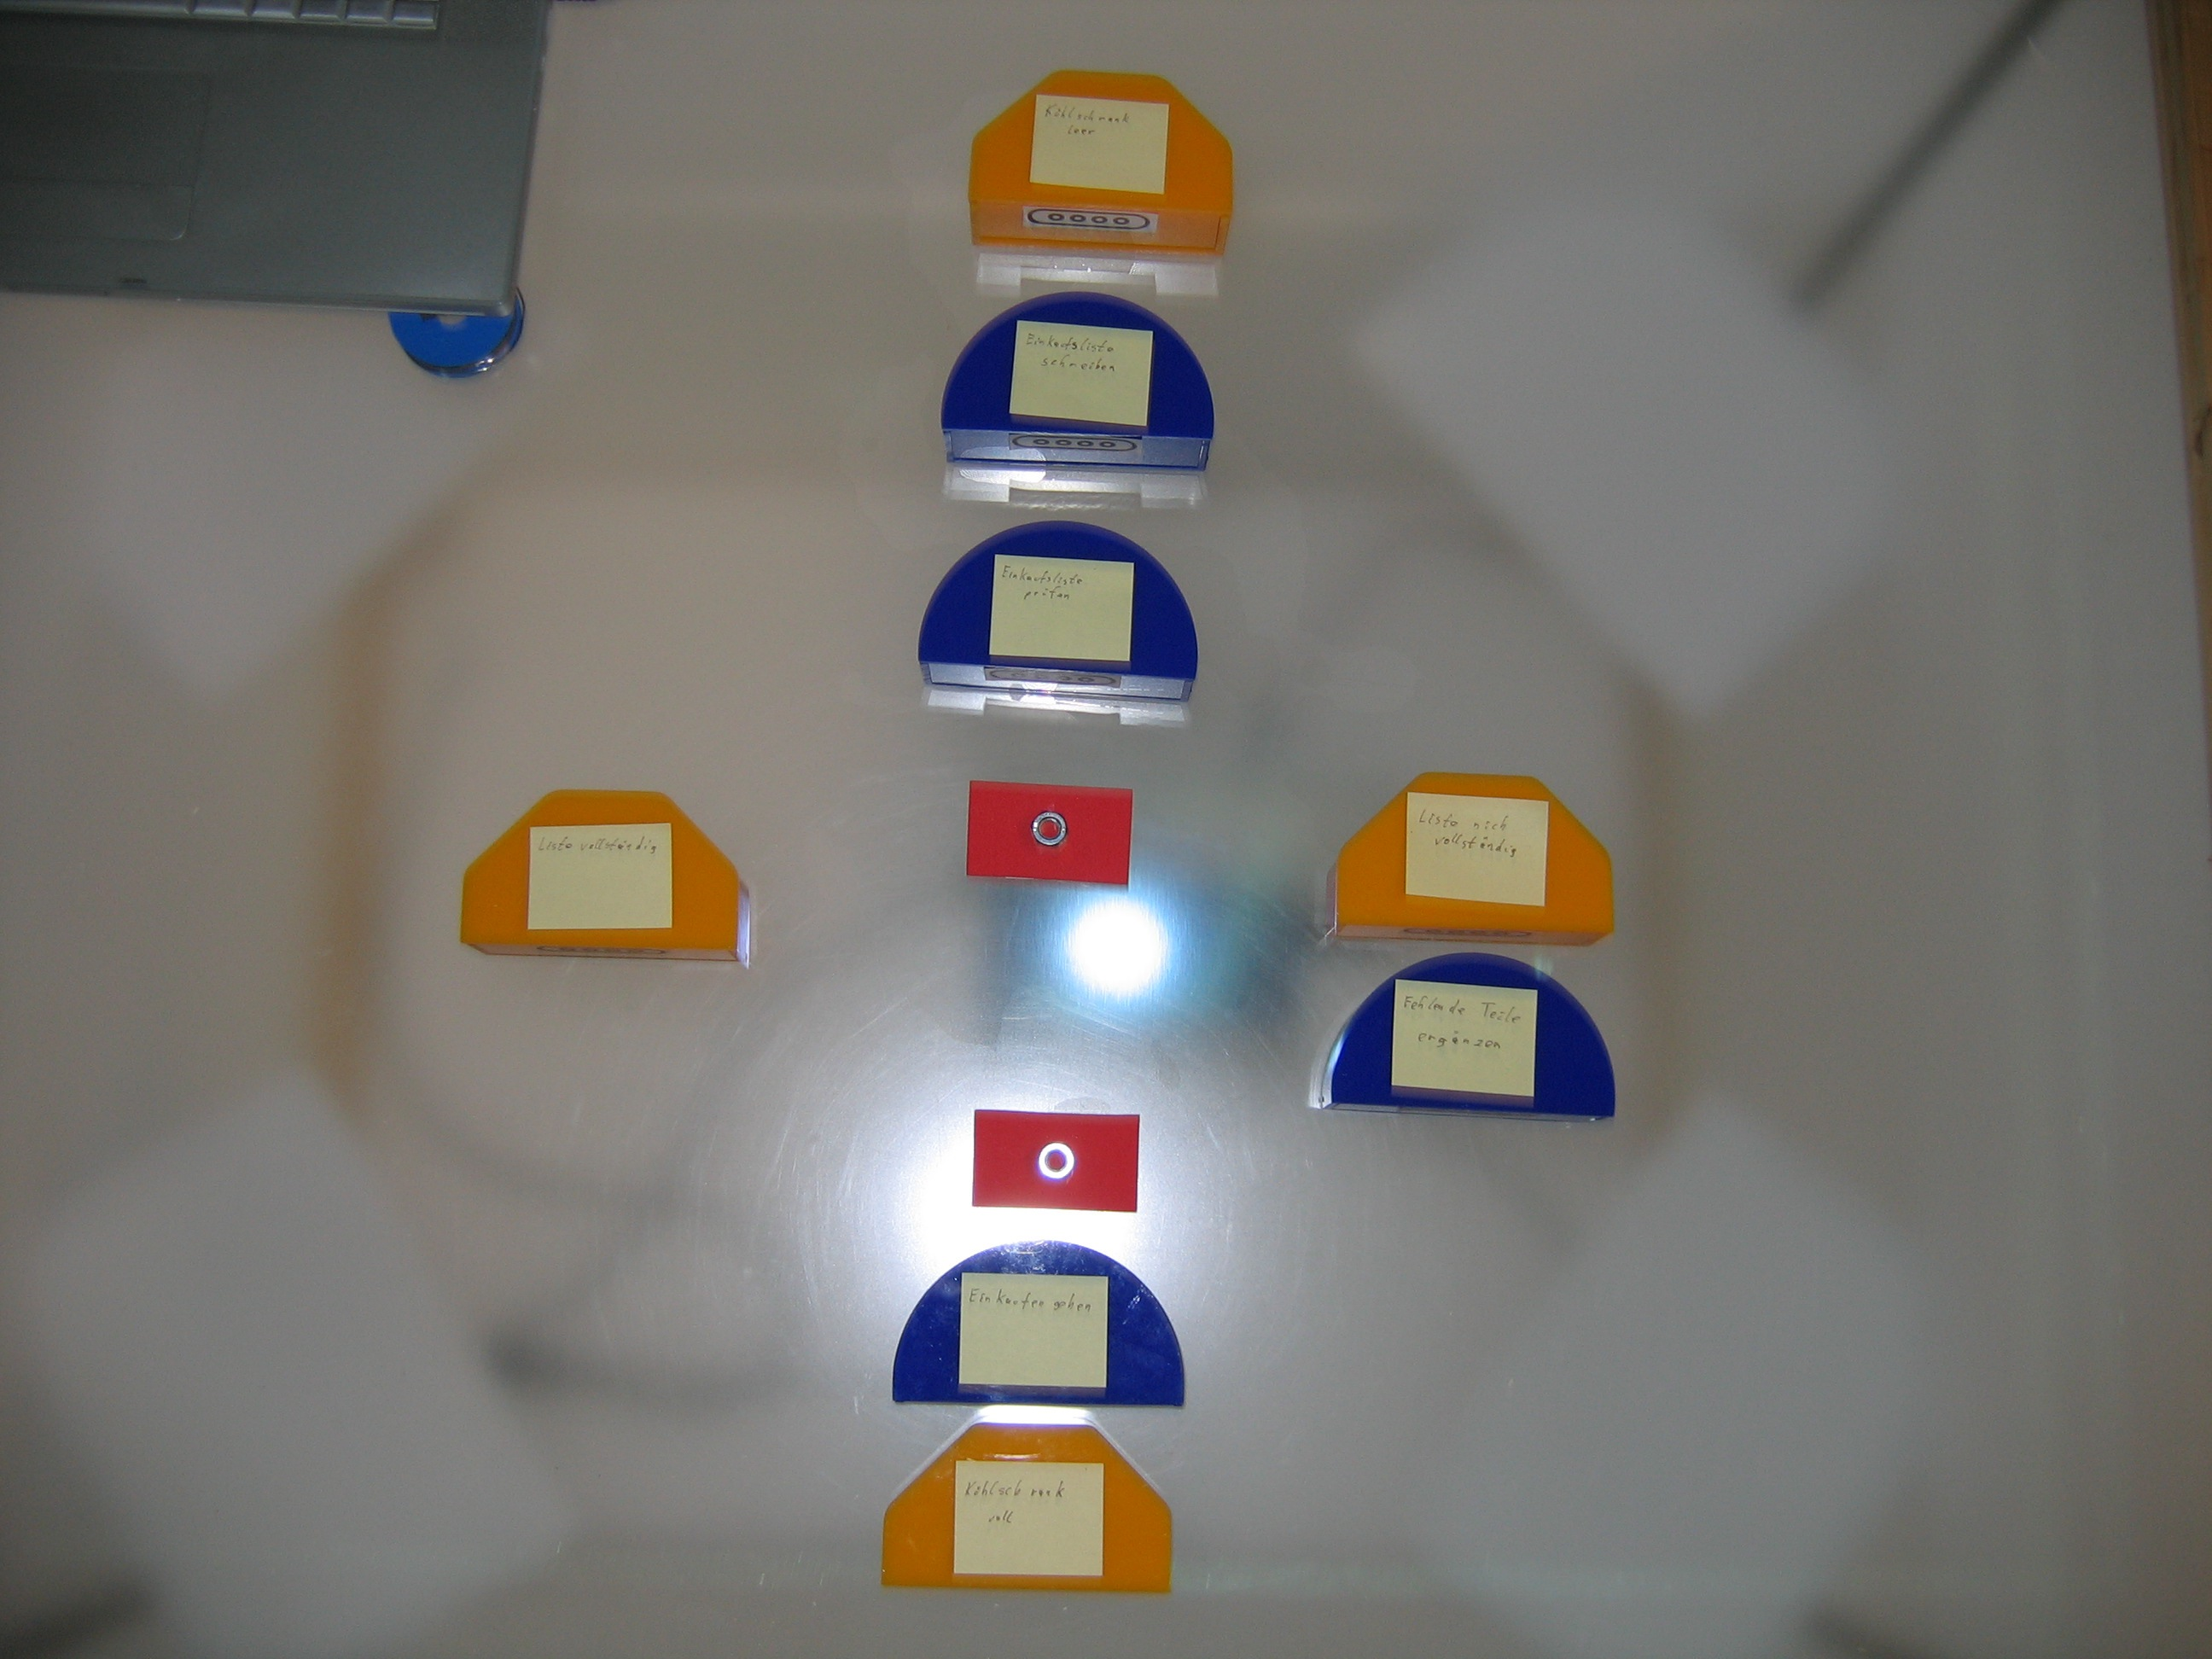
\includegraphics[width=10cm]{img/Evaluierung/modell_verbinder_unwichtig2.JPG}
	\caption{Korrekt intepretierbares Modell ohne Verbinder (ablauforientiert)}
	\label{fig:img_Evaluierung_modell_verbinder_unwichtig2}
\end{figure}

Die übrigen 46 Modelle, in denen Verbinder verwendet wurden, wurden einer nachgelagerten Interpretation durch den Leiter der Studiendurchführung\footnote{dem Verfasser dieser Arbeit} unterzogen, der an der Durchführung von 17 Modellierungsdurchgängen als Untersuchungsleiter beteiligt war (die übrigen 29 Modellierungsdurchgänge wurden im Rahmen von Diplomarbeiten erfasst, wobei die jeweiligen Diplomanden als Untersuchungsleiter auftraten). Bei dieser Interpretation wurden im ersten Schritt für jedes Modell die verwendeten Verbinder entfernt und versucht, den Modellinhalt zu interpretieren. In einem zweiten Schritt wurden die Verbinder wieder eingeblendet und die Interpretation mit dem nun vollständigen Modell verglichen. Dabei ergaben sich in 15 Fällen Unterschiede in der Interpretation, die ausschließlich auf die Verwendung von Verbindern zurückzuführen war. In den übrigen 36 Fällen explizierten bzw. bestätigten die erstellten Verbindungen die durch die räumliche Anordnung der Modellierungselemente implizit ausgedrückten Zusammenhänge. Dabei ist zu anzuführen, dass in 13 der insgesamt 46 Modelle benannte Verbinder verwendet wurden (die übrigen 33 Modelle enthielten lediglich unbenannte Verbinder). Von diesen 13 Modellen konnten 4 auch ohne die Darstellung der Verbinder korrekt (im Sinne der obigen Ausführungen) interpretiert werden. Demnach führte die Entfernung der Verbinder in 6 der 33 Modelle mit unbenannten Verbindern zu unvollständigen bzw. fehlerhaften Interpretationen. Abbildung \ref{fig:img_Evaluierung_modell_verbinder_wichtig} zeigt ein Beispiel für ein Modell, in dem die Entfernung der Verbinder zu einer unvollständigen Interpretation des abgebildeten Inhalts führte.

\begin{figure}[htbp]
	\centering
		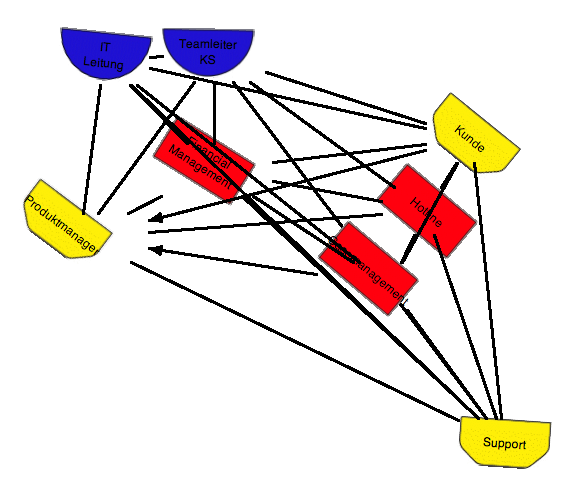
\includegraphics[width=10cm]{img/Evaluierung/modell_verbinder_wichtig.png}
	\caption{Bei Vernachlässigung der Verbinder nur unvollständig interpretierbares Modell}
	\label{fig:img_Evaluierung_modell_verbinder_wichtig}
\end{figure}

\subsubsection{Diskussion} % (fold)

Das weitgehende Fehlen von Verbindern ist in den ersten beiden Evaluierungsblöcken sowie Teilen des Evaluierungsblocks 3 auf die mangelhafte Funktion der Verbindungsherstellung durch Benutzer zurückzuführen (siehe Prüfung der Hypothese \ref{hyp:diagmodelle} in Abschnitt \ref{sub:repräsentation_diagrammatischer_modelle}). Trotzdem war es den Teilnehmenden möglich, ein gemeinsames Verständnis über die abgebildeten Zusammenhänge zu entwickeln. Auch bei der Interpretation durch Dritte, die am Entstehungsprozess des Modells nicht beteiligt waren, traten keine Missverständnisse auf. Dies gilt sowohl für ablauf-orientierte Modelle (in Evaluierungsblock 1 und 2) als auch für Concept-Map-artige Modelle (in Evaluierungsblock 3).

Insofern scheint die Hypothese bestätigt werden zu können. Diese Annahme ist insofern zu relativieren, als dass den Evaluierungsblöcken 3, 4 und 5 insgesamt 15 Modellierungsdurchgänge identifiziert werden konnten, in denen die Verwendung von Verbindungen den Modellen Bedeutung hinzufügt, die ohne diese auch implizit nicht vorhanden gewesen wäre. Eine vorbehaltslose Annahme der Hypothese erschient deshalb nicht rechtfertigbar.

Hypothese \ref{hyp:keine_verbinder} kann unter Berücksichtigung der obigen Ausführungen damit nicht bestätigt werden. Während in vielen Fällen die ausschließliche räumliche Anordnung von Modellierungselementen ausreichend zu sein scheint, um die beabsichtigte Bedeutung zu kommunizieren, konnten Fälle identifiziert werden, in denen dies nicht möglich war.

\subsubsection{Ergebnis} % (fold)

\textbf{Die Hypothese \ref{hyp:keine_verbinder} kann auf Basis der Untersuchung nicht bestätigt werden.} Während zu Bildung eines einheitlichen Verständnisses in vielen Fällen die implizite Abbildung von Zusammenhängen durch räumliche Konfiguration der Modellierungselemente ausreichend erscheint, konnten Fälle identifiziert werden, in denen die explizite Repräsentation von Verbindern dem Modell Bedeutung hinzufügte, die ohne Darstellung derselben nicht kommunizierbar gewesen wäre.

% subsection abbildung_von_zusammenhängen_ohne_verbinder (end)
% section m_ergebnisse (end)

\section{Zusammenfassung} % (fold)
\label{sec:m_zusammenfassung}

In diesem Kapitel wurde die Evaluierung des Aspektes der Modellierung mit dem hier vorgestellten Werkzeug beschrieben. Die hier betrachteten Hypothesen beschäftigen sich mit dem Modellierungsergebnis an sich sowie dem Prozess der Modellerstellung. In Abgrenzung dazu wurde in Kapitel \ref{cha:eval_werkzeug} die Verwendung des Werkzeugs im Allgemeinen sowie dessen Verständlichkeit geprüft. Kapitel \ref{cha:eval_aw} beschäftigt sich hingegen mit der Rückwirkung der Modellierung bzw. der Modelle auf die eigentlichen Betrachtungsgegenstände (also etwa operative Arbeitsabläufe).

Im Rahmen dieses Kapitels wurden drei aus der Aufgabenstellung begründbare Hypothesen und eine explorativ während der Evaluierung gebildete Hypothese getestet. Die ersten beiden Hypothesen beschäftigen sich mit einer eventuell einschränkenden Wirkung des Werkzeugs auf die Modellbildung. Wie in den Anforderungen \ref{anf:nicht_vorgegebene_semantik_der_modellierungselemente} und \ref{anf:bearbeitung_von_beliebig_komplexen_modellen} formuliert, muss das Werkzeug zur Unterstützung von „Articulation Work“ einerseits semantische Offenheit bei der Modellierung bieten (d.h. die Modellierenden nicht bei der Abbildung der eigenen Konzeptualisierung des abzubildenden Sachverhaltes einschränken) und andererseits die Abbildung beliebig umfangreicher Modelle erlauben. 

Hypothese \ref{hyp:keine_einschränkung} („Semantische Offenheit“) konnte dabei insofern bestätigt werden, als dass die Teilnehmenden das Werkzeug nur in Einzelfällen als semantisch einschränkend empfanden. Der Vergleich mit einem semantisch vollständig offenen Werkzeug, dass die Anzahl der Elementtypen im Gegensatz zum vorliegenden Werkzeug nicht beschränkt, deutet jedoch darauf hin, dass in manchen Anwendungsfällen tatsächlich mehr als die drei im Werkzeug semantisch belegbaren Elementtypen zum Einsatz kommen sollten.  

Hypothese \ref{hyp:beliebige_komplexität} („Beliebiger Modellumfang“) konnte im Rahmen der Untersuchung nicht bestätigt werden. Die beschränkte Größe der Modellierungsoberfläche scheint einschränkend auf den Modellumfang zu wirken, die Möglichkeit der Einbettung von Teilmodellen ist dabei kein adäquater Ersatz. In einer vergleichenden Studie mit einem die Arbeitsfläche nicht beschränkenden Werkzeug wurden bei identischer Aufgabenstellung im Durchschnitt Modelle mit doppelten Umfang als auf dem hier vorgestellten Werkzeug erstellt. Auch die Rückmeldungen der Teilnehmenden deuten darauf hin, dass die Beschränkung der Modellierungsoberfläche in vielen Fällen als einschränkender Faktor wahrgenommen wird.

Hypothese \ref{hyp:historie} („Reflexion des Modellierungsverlaufs“) untersucht, ob die Verfügbarkeit der Modellierungshistorie einen positiven Einfluss auf die Nachvollziehbarkeit des Modellinhaltes hat. Diese Hypothese konnte im Rahmen der Untersuchung bestätigt werden. Einschränkend ist jedoch anzumerken, dass die Korrektheit der Interpretation vor allem in Fragestellungen, die zu ablauforientierten Modellen führen, in vielen Fällen eher gering ist. Es ist daher fraglich, ob eine Interpretation ausschließlich auf Basis der gespeicherten Repräsentationen des Modells ausreichend ist bzw. zu qualitativ zufrieden stellenden Ergebnissen führt.

Hypothese \ref{hyp:stärkere_kooperation} („Stärkere Kooperation“) untersucht, ob die Verwendung des Werkzeugs zu stärkerer Kooperation führt als die Verwendung eines bildschirmbasierten Werkzeugs. Diese Hypothese konnte im Rahmen der Untersuchung bestätigt werden. Die Verwendung des Werkzeugs führt im Vergleich zur Anwendung eines bildschirm-basierten Werkzeugs zu einem signifikant höheren Anteil an Diskussion während der Modellbildung und zu ausgeglichenerer physischer Beteiligung am Modellierungsvorgang zwischen den Teilnehmern. Die Daten aus der Befragung der Teilnehmer stärken die Hypothese zwar nicht signifikant, zeigen aber eine leichte Tendenz zu deren Bestätigung. 

Die letzte in diesem Kapitel untersuchte Hypothese (Hypothese \ref{hyp:keine_verbinder}, „Verbinder nicht notwendig“) betraf die explorativ gebildete Vermutung, dass zur Repräsentation von Zusammenhängen in Modellen die explizite Darstellung von Verbindern nicht notwendig wäre sondern die ausschließliche räumliche Konfiguration der Modellierungselemente zueinander ausreichen würde, um die Zusammenhänge erfassbar zu machen. Während dies im überwiegenden Teil der Anwendungsfälle möglich war, konnten Modelle identifiziert werden, in denen die Verbinder Information codierten, die rein durch die räumliche Anordnung der Modellelemente nicht ableitbar gewesen wäre (in etwa 25\% der Fälle). Hypothese \ref{hyp:keine_verbinder} konnte im Rahmen der Untersuchung damit nicht bestätigt werden.

Insgesamt zeigt sich damit, dass das Werkzeug nur eingeschränkt zur Abbildung diagrammatische Modelle geeignet ist. Im Sinne der Zielsetzung dieser Arbeit -- der Unterstützung von „Articulation Work“ -- ist dies jedoch nur von eingeschränkter Wichtigkeit. Vielmehr steht die Unterstützung der Kommunikation zwischen den beteiligten Individuen und der Abgleich derer mentaler Modelle im Vordergrund. Die Ergebnisse deuten darauf hin, dass das Werkzeug diesen Ansprüchen gerecht wird. Im nächsten Kapitel wird nun untersucht, inwieweit der Abgleich tatsächlich stattfindet (also „Articulation Work“ erfolgreich durchgeführt werden konnte) und welche Auswirkungen dies auf die Arbeitsrealität hat.

% section zusammenfassung (end)
% chapter eval_modell (end)